\documentclass{DeustoFDP}
\emergencystretch=1em % this is for using emergency stretches in overfulls
\usepackage[toc, acronym, nomain]{glossaries}
\usepackage{eurosym}
\usepackage{verbments}
\listofpyglistingsname{Algorithm Index}

\hypersetup{
	pdfauthor={Iban Eguia Moraza},
	pdftitle={Remote robotic experiment integration in a game platform to promote STEM in young people},
}

\bibliography{bibliography}
\makeglossaries
\chapter*{Acronyms}
\addcontentsline{toc}{chapter}{Acronyms}

\begin{itemize}
	\item \textbf{STEM}: Science, Technology, Engineering and Mathematics

	\item \textbf{GOLC}: Global Online Laboratory Consortium

	\item \textbf{MIT}: Massachusetts Institute of Technology

	\item \textbf{VISIR}: Virtual Instrumentation Systems In Reality

	\item \textbf{IDE}: Integrated Development Environment

	\item \textbf{API}: Application Programming Interface
\end{itemize}


\begin{document}

\frontmatter
\pagestyle{plain}

\begin{titlepage}
  \newgeometry{left=0cm,right=0cm,bottom=0cm,top=0cm}\thispagestyle{empty}
  \includegraphics{fig/frontpage_comp}
  \restoregeometry
\end{titlepage}
\cleardoublepage

\chapter*{Abstract}

Responding to the strong growing demand of new learning tools, a new learning experience is
presented, based on remote laboratories. This project, tries to create what at our best knowledge
will be the first game platform based on remote laboratories to introduce young students between 10
and 18 years old to \acrshort{stem} (\acrlong{stem}) in an enjoyable way.

The game platform will be divided in two main scenarios. The first of them will be a trivial type
game, where the user will be able to control a robot in a labyrinth and answer some questions that
will give points to the user. Winners will be given a prize. Moreover, in this scenario, a
psychology experiment will be performed, aiming to help in the fight against pseudoscience.

The second scenario will be a service in which the user will be able to program the robot from a
visual \acrshort{ide} (\acrlong{ide}). This will teach students the basics of programming by letting
them use blocks to program the robot and see the result.

\vspace{2em}

{\Large\bfseries\sffamily Keywords}
\vspace{3\medskipamount}

Remote Laboratories, WebLab-Deusto, Serious Games, Psychology, Pseudoscience


\cleardoublepage\tableofcontents
\cleardoublepage\listoffigures
\cleardoublepage\listoftables
\cleardoublepage\listofpyglistings

\mainmatter
\pagestyle{phdthesis}

\chapter{Introduction}

\section{Background}

% TODO: insert images

\subsection{Remote Laboratories}

Remote laboratories are usual laboratories, with the peculiarity that they can be accessed through
the Internet~\cite{remote_labs}. They give students the option to use the laboratory even from home
or while the university or school is closed. This means that the students are able to do their
homework or experimentation using the equipment at their school or university without the need for
them to be physically there.

Currently they are becoming more popular due to the competitive advantage they can give to schools
and universities. Since there is no need for the student to be physically in the laboratory, the
laboratory does not need to be physically in the school or university, giving the option to share
laboratories between institutions and thus giving important economic benefits without reducing
the practice time of the students, or even increasing it.

\subsection{Serious Games}

Serious games are video games that do not only entertain, but they manage to teach. Thanks to that,
they can be used to improve the quality of the learning environment for students. Moreover, since
games in many cases attract better the attention of young people, they can even be a better tool for
teaching, at least, the basic concepts of some subjects.

\subsection{WebLab-Deusto}

WebLab-Deusto is a remote laboratory facility located in the University of Deusto~\cite{weblab},
Bilbao. Since 2001, it has been providing students with remote laboratories to complete their
academic learnings. Since then, it has been extended and many of it's laboratories is available
all over the world. It's no longer a laboratory only made for microelectronics university students
since nowadays it serves schools and universities everywhere to provide them with remote
laboratories.

Among others, it serves an experiment to prove and measure the Archimedes' principle, an experiment
to program and control a robot and some microelectronics experiments with PLDs and FPGAs. Moreover,
there are more laboratories in development, such as an elevator to teach students how to program and
control them, an experiment with an aquarium where students can give them food and, of course, the
project presented here: a complete learning experience given by a robot.

\section{Motivation}

Technology is changing every day, and among other luxuries, it gives us the ability to improve the
way we perform our tasks. Nowadays, one of the most important things in our lives, that consumes
more than a quarter of it is our education. In a strong belief that technology can contribute to
give future generations better tools for learning, serious games seem to be a viable option I would
like to deepen. Having the opportunity to do so in a remote environment such as Weblab-Deusto gives
us the ability to create a remote laboratory, with the potential for being used by many people
around the world, and thus make a difference in learning environments.

\chapter{Background and Rationale}

\section{Background}

This project aims to create a serious game based on a robot in a remote laboratory. Moreover, it
aims to create a complete visual programming experience to teach the basics of programming. Thus,
in this state of the art, We will cover the three main topics that the project uses as a base and we
will deepen into them.

\subsection{Remote Laboratories}

Remote laboratories are usual laboratories, with the peculiarity that they can be accessed through
the Internet~\cite{remote_labs}. They give students the option to use the laboratory even from home
or while the university or school is closed. This means that the students are able to do their
homework or experimentation using the equipment at their school or university without the need for
them to be physically there.

Currently they are becoming more popular due to the competitive advantage they can give to schools
and universities. Since there is no need for the student to be physically in the laboratory, the
laboratory does not need to be physically in the school or university, giving the option to share
laboratories between institutions and thus giving important economic benefits without reducing
the practice time of the students, or even increasing it.

Thus, remote laboratories can be really helpful in teaching main concepts about science and
technology. The next laboratories are the most known ones that are working with science and
technology.

\subsubsection{Global Online Laboratory Consortium}

The \acrlong{golc} or \acrshort{golc} is an organization that focuses on the promotion of the
development of remote laboratories for educational use. They commonly promote remote laboratories
through conferences~\cite{golc1st}. They also support and encourage the sharing of these
laboratories between institutions.

For promoting laboratories, they created an award (Figure~\ref{fig:golc_award}) for remote
experimentation and another one for simulated experimentation.

\begin{figure}[!htbp]
	\centering
	\includegraphics[width=0.5\textwidth]{fig/golc_award}
	\caption{\acrshort{golc} Online Laboratory Award 2015}\label{fig:golc_award}
\end{figure}

\subsubsection{WebLab-Deusto}

WebLab-Deusto is a remote laboratory located at the University of Deusto, Bilbao. There are multiple
types of laboratories there, and all is being controlled by a software they developed, called
WebLab. Moreover, Pablo Orduña, one of it's main researches developed a complete federation model
to be able to share laboratories across the world~\cite{porduna_phd}.

In WebLab-Deusto they created one of the most used remote laboratories in electronics teaching. It
is called \acrshort{visir}~\cite{visir}, and it recreates circuits made visually by students in real
hardware so that students can take real measurements.

\begin{figure}[!htbp]
	\centering
	\includegraphics[width=0.5\textwidth]{fig/weblab}
	\caption{WebLab-Deusto logo.}
\end{figure}

\subsubsection{iLab Project at \acrshort{mit}}

The \acrlong{mit} has its own remote laboratory platform called iLab. They
have many remote laboratories where they experiment with Dynamic Signal Analyzers, Heat Exchangers
and even with Polymer Crystallization. It has even inspired some big projects using this technology
such as an on-line repository to locate remote laboratories~\cite{ilabs_multi}.

\begin{figure}[!htbp]
	\centering
	\includegraphics[width=0.5\textwidth]{fig/icampus}
	\caption{iCampus logo, project at \acrshort{mit} where iLabs have been created.}
\end{figure}

\subsubsection{Robotic remote experiments}

Some of the laboratories listed before have currently implementations of robotic experiments in
as a teaching material in some areas. In WebLab-Deusto, for example, they have what they call
WebLab-Bot (Figure~\ref{fig:weblab-bot}). This robot is based on Azkar-Bot robot and it is used for
electronic students to learn how to program it. They have simple demonstrations that follow a black
line or respond to simple commands.

\begin{figure}[!htbp]
	\centering
	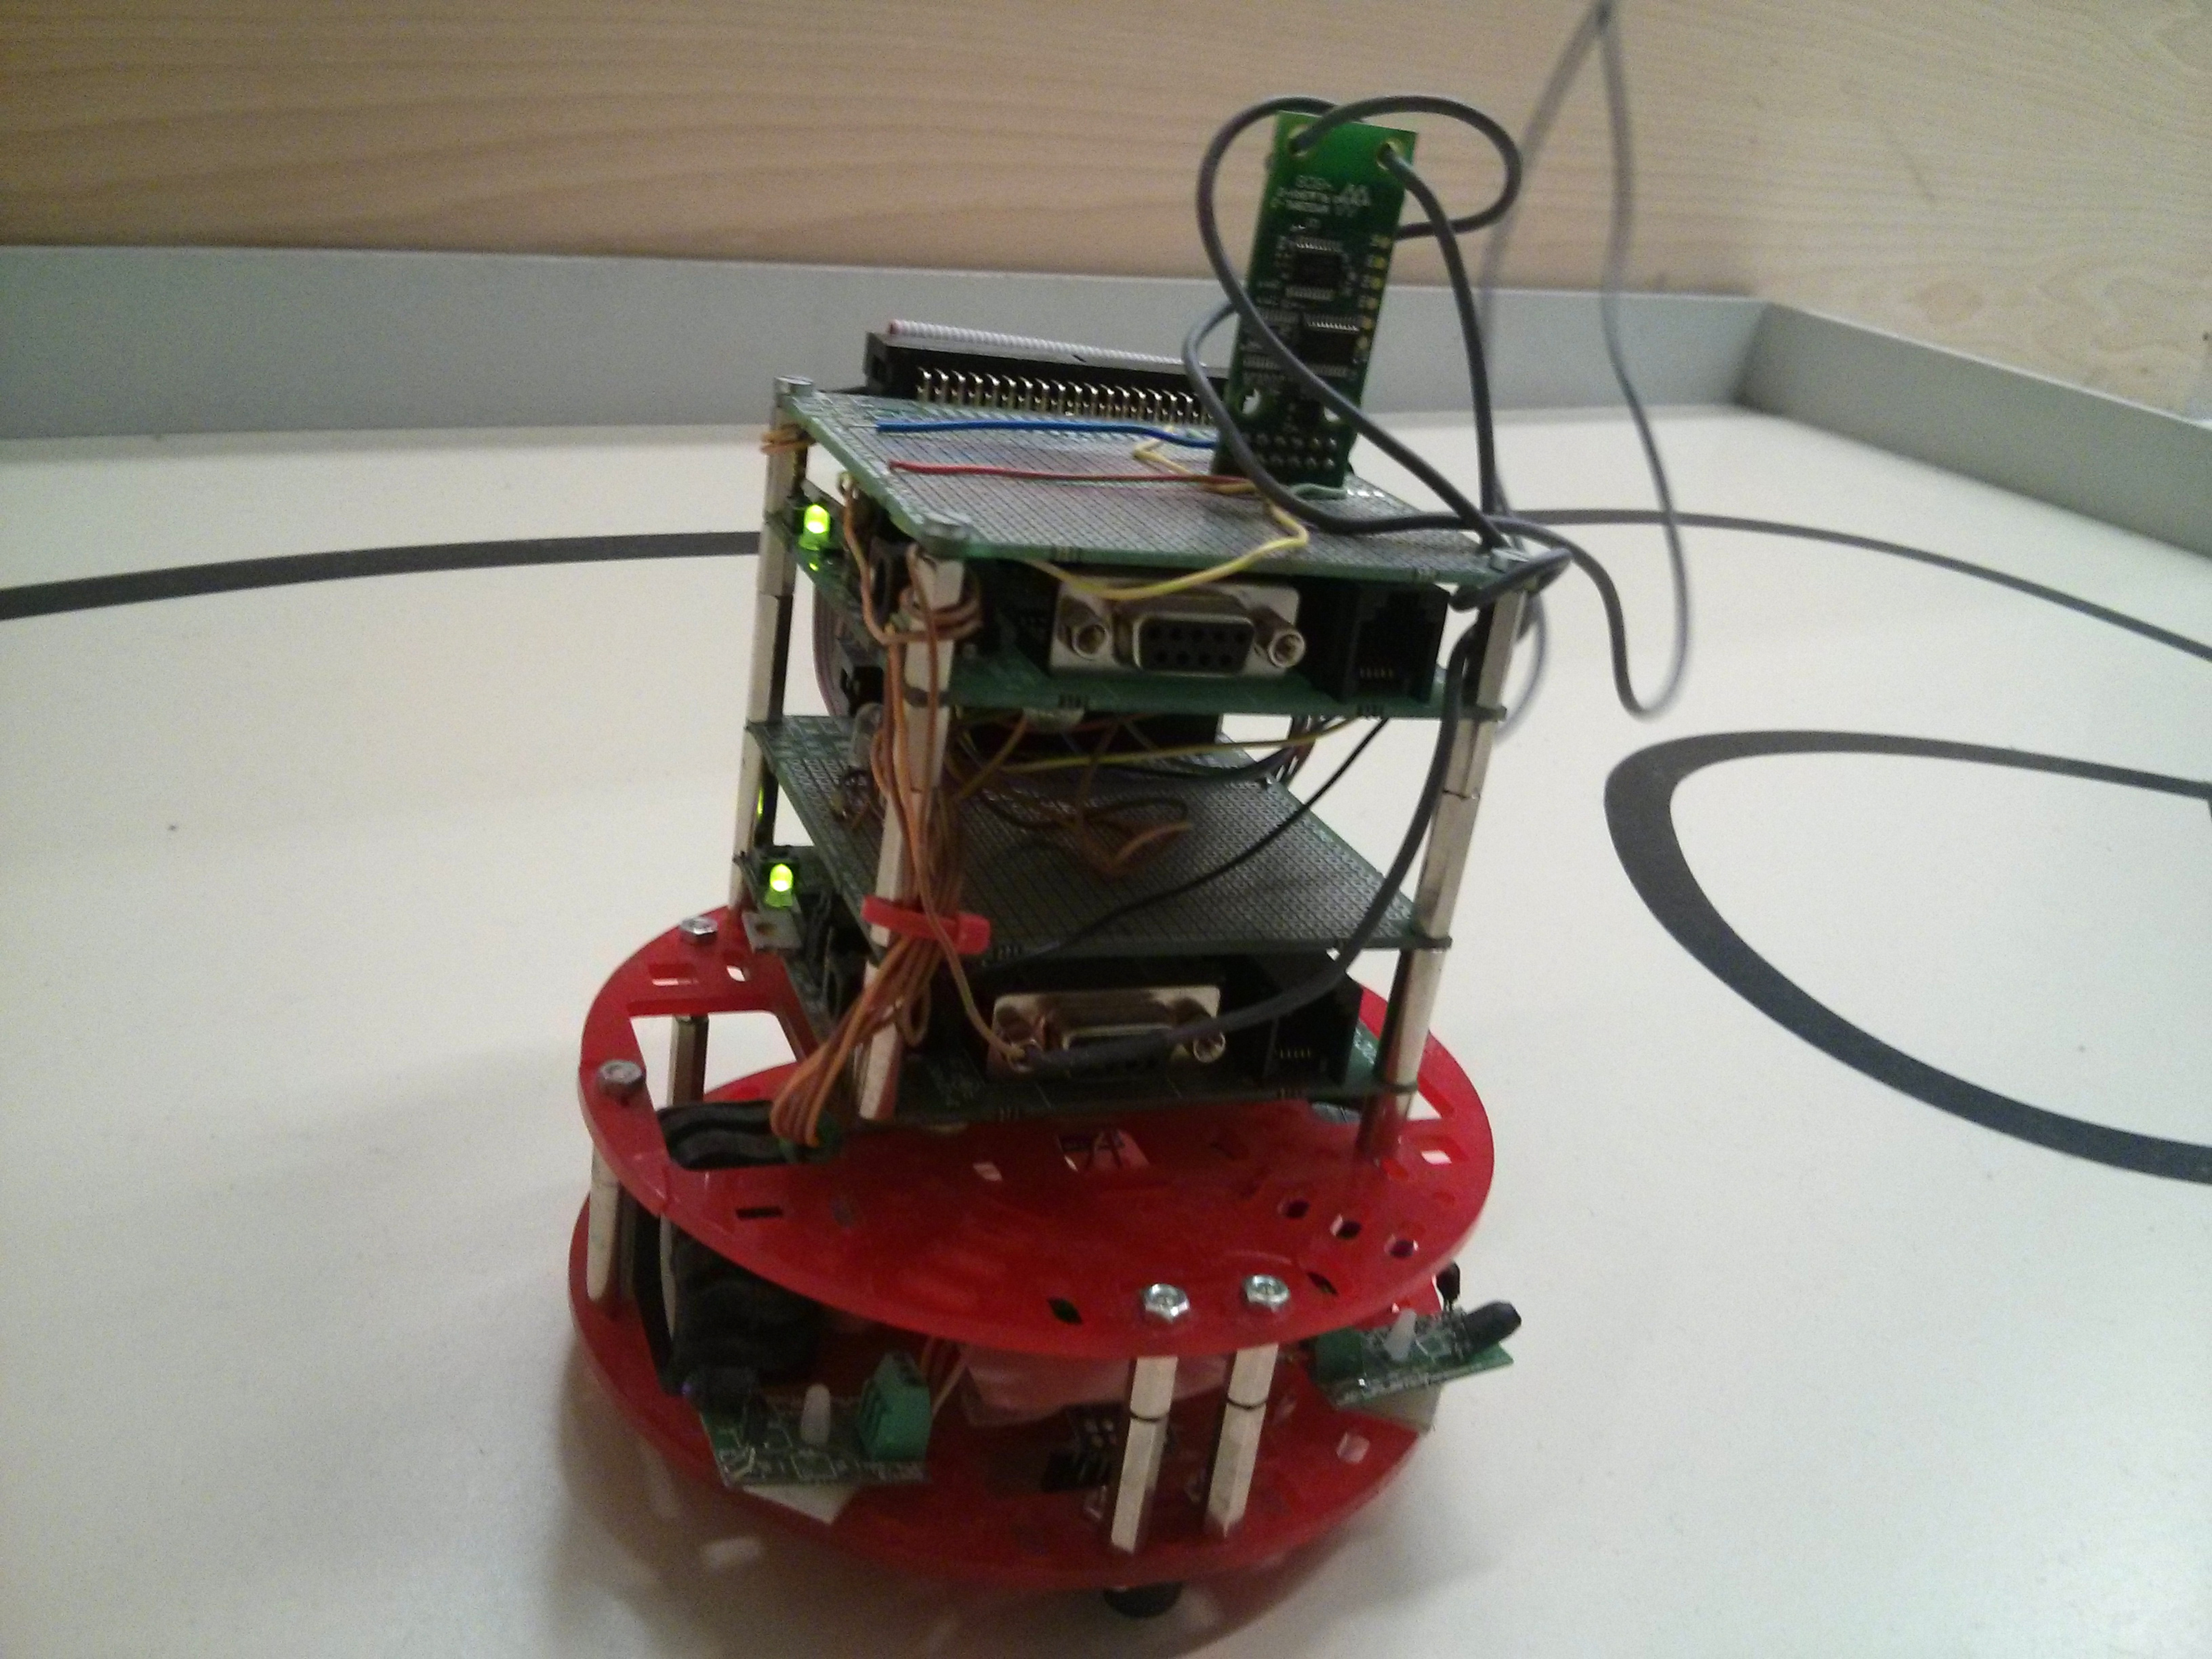
\includegraphics[width=0.5\textwidth]{fig/weblab-bot}
	\caption{WebLab-Bot, a robot based on Azkar-Bot as a remote laboratory in WebLab-Deusto.}
	\label{fig:weblab-bot}
\end{figure}

Moreover, in The Labshare Institute, they have a robot called iRobot, that teaches how to deal with
accuracy of sensors, localization and mapping. Finally, the robot that will be used in this
project is called Romie (Figure~\ref{fig:labyrinth}. It is located in WebLab-Deusto and it has the
needed functionality for this project: it is capable of following a line, it detects walls and it
detects intersections. We have built a complete labyrinth for it where we will deploy this project.

\begin{figure}[!htbp]
	\centering
	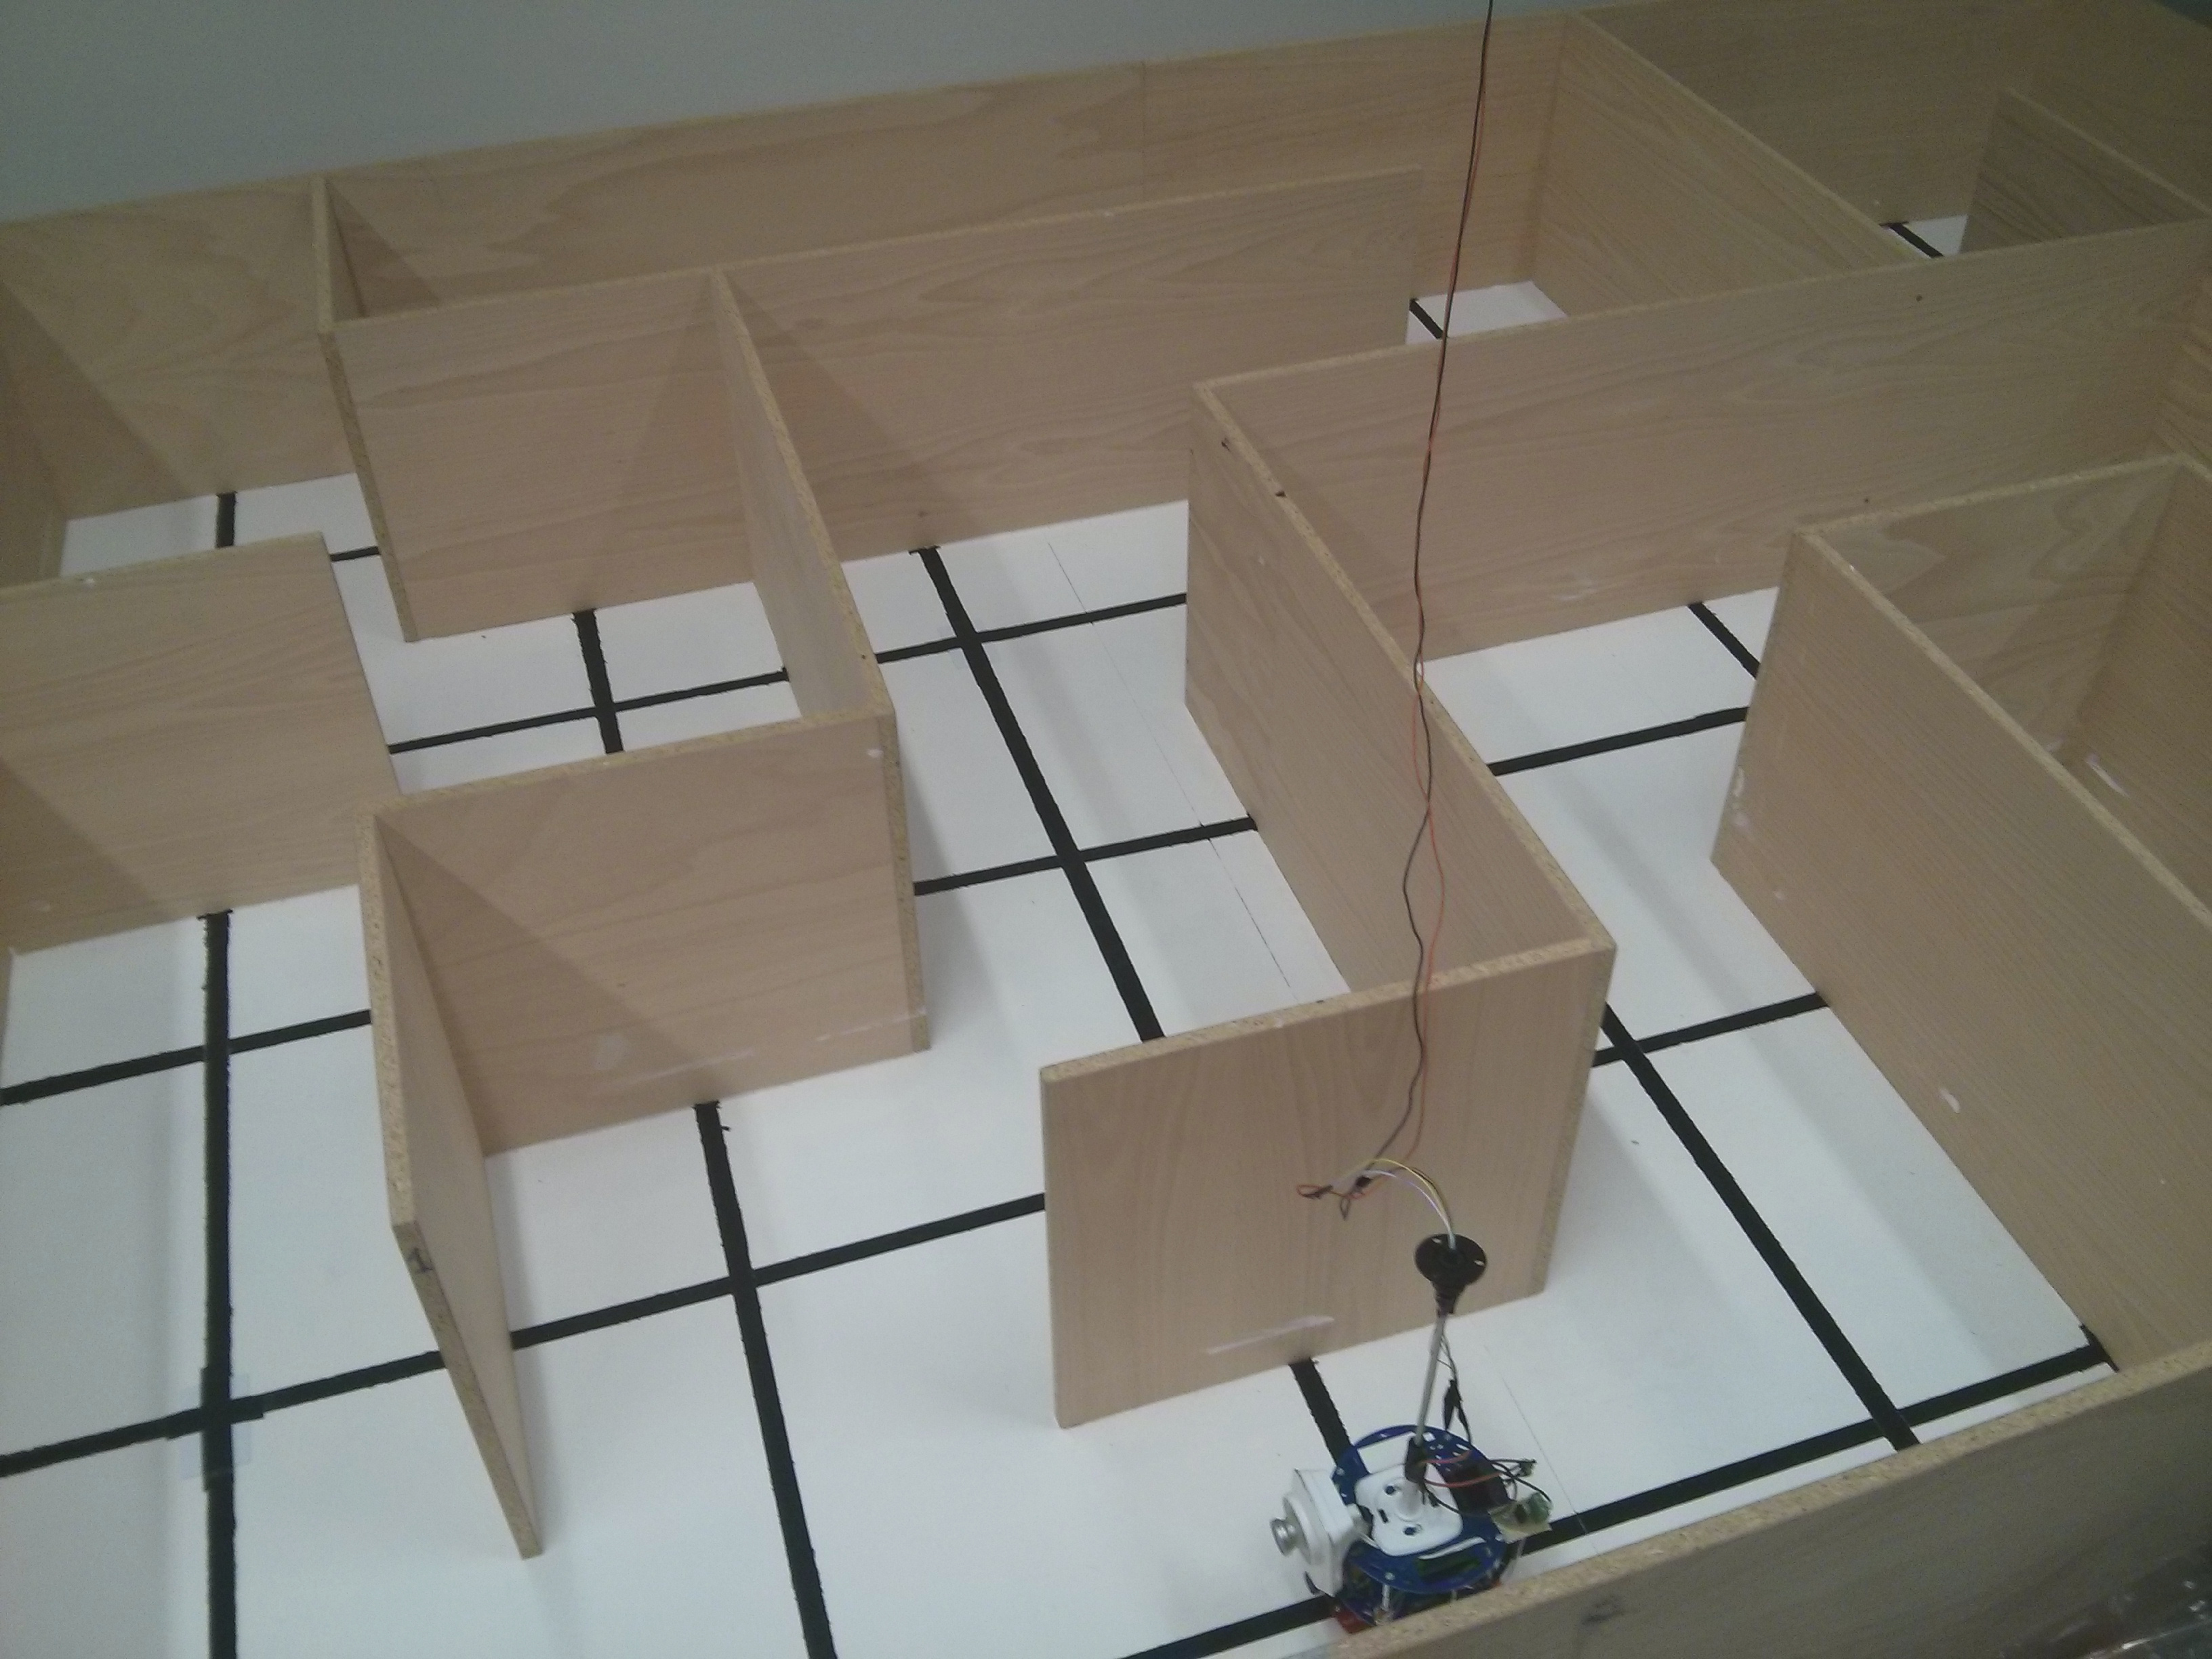
\includegraphics[width=0.5\textwidth]{fig/labyrinth}
	\caption{Romie, the robot we will be using in this project in its labyrinth.}\label{fig:labyrinth}
\end{figure}

\subsubsection{Simulations}

Even if the project will not be based on simulated robotics but in real robots, currently many
many projects use simulations to bring some of the experience to users. A simulation is usually
less costly than a remote laboratory, since not much hardware is required. On the other hand,
students will not be using real tools and experimentation environments, so the experience of using
them will not be as complete as in a remote laboratory.

Nevertheless, some prefer creating hybrid laboratories~\cite{hybrid_labs}. In these cases, the
laboratories add a simulation layer over the real laboratory. This way, the user still uses a real
laboratory, with the benefits of knowing how to use the laboratory and doing real experimentation,
and it also gives the user some more benefit by simulating extra conditions that could be expensive
to create in a real laboratory.

\subsection{Serious Games and Visual Programming}

Serious games are video games that do not only entertain, but they manage to teach. Thanks to that,
they can be used to improve the quality of the learning environment for students. Moreover, since
games in many cases attract better the attention of young people, they can even be a better tool for
teaching, at least, the basic concepts of some subjects. For our purpose here, we will analyze the
most known tools for visual programming environments.

Visual programming is a way of programming that instead of using real code in a real programming
language uses a visual interface to create programs and then translate them to a well known
language. This way, people that are not yet used to programming languages, interfaces such as
\acrshort{ide}s or code execution, and do not understand the basis of programming can start learning
by using a simple visual environment~\cite{visual_programming}.

\subsubsection{Scratch}

Scratch is one of the most known visual programming tools~\cite{scratch}. It is in itself an
\acrshort{ide}, made by the \acrshort{mit} to help to teach programming to inexperienced users. It
teaches the basic concepts of algorithms and it gives an enough powerful tool so that users can
enjoy using it. It's main concept is to join basic programming blocks so that functionality is
created.

Moreover, they have created a complete collaboration platform where all the users of Scratch can
share their creations and check out the ones that others have made. That way, users can learn more
by looking at code created by others.

\subsubsection{Blockly}

Blockly, unlike Scratch, is not a visual programming \acrshort{ide}, but a visual programming
library to create visual programming editors and \acrshort{ide}s. It has the same basis as Scratch,
so it contains basic programming blocks to build applications by joining them
(Figure~\ref{fig:blockly}), and it also gives developers the option to create their own blocks with
a simple \acrshort{api}. It was created by Google and it's source is now available in GitHub.

\begin{figure}[!htbp]
	\centering
	\includegraphics[width=0.5\textwidth]{fig/blockly}
	\caption{Simple program example created in Google's Blockly.}\label{fig:blockly}
\end{figure}

Blockly enables developers to create their own programming environments for their projects, so they
can adapt Blockly itself to their needs, and thus, making it possible for them to even create
complete \acrshort{ide}s for their projects based on visual programming.

\subsection{WebLab-Deusto}

WebLab-Deusto is a remote laboratory facility located in the University of Deusto~\cite{weblab},
Bilbao. Since 2001, it has been providing students with remote laboratories to complete their
academic learnings. Since then, it has been extended and many of it's laboratories is available
all over the world. It's no longer a laboratory only made for microelectronics university students
since nowadays it serves schools and universities everywhere to provide them with remote
laboratories.

Among others, it serves an experiment to prove and measure the Archimedes' principle
(Figure~\ref{fig:archimedes}), an experiment to program and control a robot and some
microelectronics experiments with PLDs and FPGAs. Moreover, there are more laboratories in
development, such as an elevator to teach students how to program and control them, an experiment
with an aquarium where students can give them food and, of course, the project presented here: a
complete learning experience given by a robot.

\begin{figure}[!htbp]
	\centering
	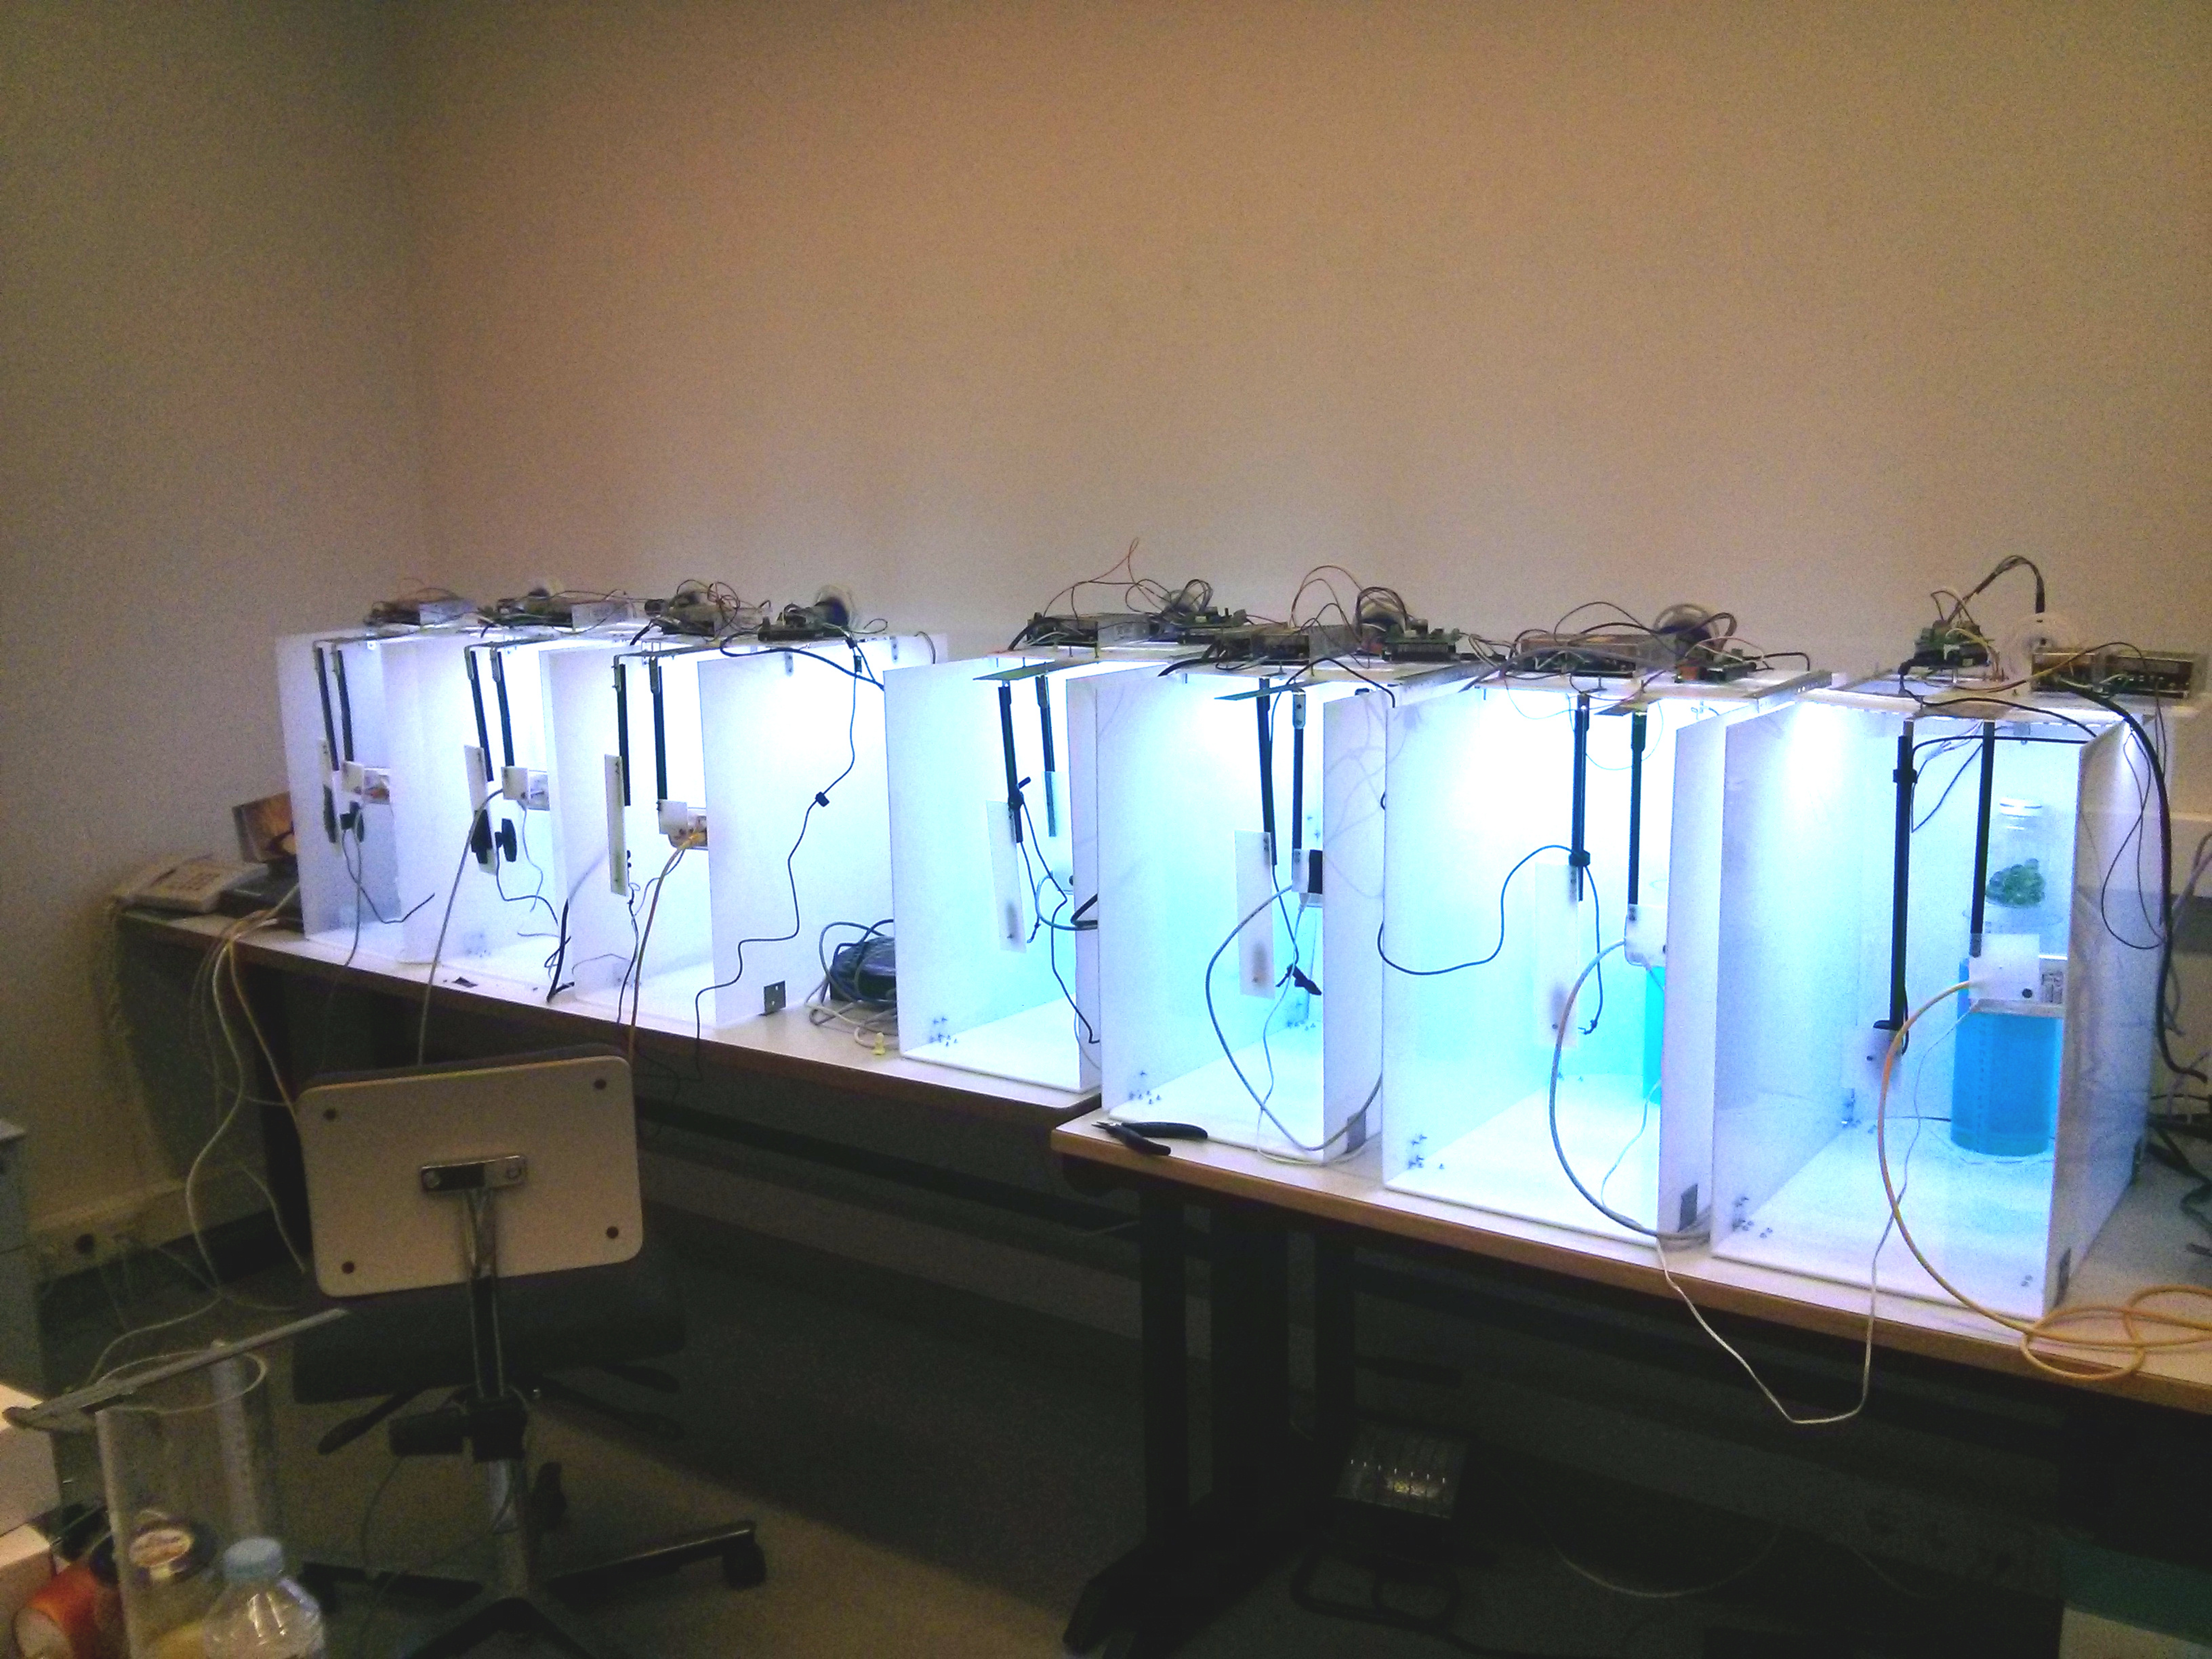
\includegraphics[width=0.5\textwidth]{fig/archimedes}
	\caption{Archimedes experiment in WebLab-Deusto.}\label{fig:archimedes}
\end{figure}

\section{Rationale}

Technology is changing every day, and among other luxuries, it gives us the ability to improve the
way we perform our tasks. Nowadays, one of the most important things in our lives, that consumes
more than a quarter of it is our education. In a strong belief that technology can contribute to
give future generations better tools for learning, serious games seem to be a viable option I would
like to deepen. Having the opportunity to do so in a remote environment such as WebLab-Deusto gives
us the ability to create a remote laboratory, with the potential for being used by many people
around the world, and thus make a difference in learning environments.

\chapter{Objectives and Scope}

The platform will integrate sophisticate hardware and software elements that allow us to deploy a
remote controlled robot so that it can be used by students in a game platform using the provided
user interface.

The development of the project will require knowledge about the hardware (for the maintenance and
modifications of the robot), knowledge about communication protocols (\acrshort{http},
\acrshort{tcp}/\acrshort{ip} and Bluetooth) for command and image transmission, knowledge about web
engineering (for the develoment of the client and the interaction with the WebLab-Deusto platform)
and user interface design knowledge for creating a user-friendly interface taking into account the
requirements asked by \acrshort{fecyt} Remote Science.

The secondary objectives of the project will be the following:
\begin{itemize}
\item \textbf{Requirement analysis, state of the art study. Requirements specification}:

A complete state of the art study will be performed to know th current market situation regarding to
remote robotic laboratories and the \acrshort{stem} promotion in young people. Moreover, a
requirement analysis will be performed which will give us the final requirement specification.

\item \textbf{\acrshort{stem} element revision for young students}:

We will analyze which are the most influential elements in the education of students in the
\acrshort{stem} area so that they can be maximized when developing the platform. They will be proved
with young students aged between 10 and 18 years old.

\item \textbf{Current hardware platform analysis and modification}:

We will study the possibilities of the current hardware in WebLab-Deusto (the robot Romie) and the
needed changes will be developed to adapt it to the needs of the project.

\item \textbf{\acrshort{api} for remote control}):

A complete control \acrshort{api} will be developed, able of communicating with the robot with a
a simple interface for the client software taking into account the restrictions of the WebLab-Deusto
environment.

\item \textbf{Trivial type game platform development - registration, game design, score and robot
control}:

A game platform will be created based on a simple trivial game, where the user will have to answer
the proposed questions to obtain a high score. A contest will take place where these users will get
a prize. Game rules must be carefully analyzed so that the game will not be too easy nor too
difficult.

\item \textbf{Integration of a psychological experiment for fighting against pseudoscience. Work
with a psychologist group}:

The psychology laboratory of the University of Deusto, Labpsico will provide an experiment about the
fight against pseudoscience that will be added to the game in one of its game modes. The relevant
data for the psychological research will be sent to Labpsico, while the user will receive a bonus in
the game depending on his or her performance in the psychological activity.

\item \textbf{Visual programming environment for the robot}:

A visual programming environment for the robot will be created based on one of the most known
platforms: Blockly or Scratch, still to be decided, depending on the previous research. This
environment will be used to teach the basics of programming to young students.

\item \textbf{Integration in WebLab-Deusto}:

We will use the WebLab-Deusto platform provided by the University of Deusto so that we can deploy
the experiment in a production environment along with the rest of the experiments. This provides the
experiment with a simple interface for the communication with the experiment server and with the
robot. It will also be in charge of managing user queues and user authentication.

\item \textbf{Platform dissemination: Deployment in the ``Ciencia Remota'' project of
\acrshort{fecyt} and testing by students}:

The game will be deployed in th ``Ciencia Remota'' projct of \acrshort{fecyt} where many
institutions work to bring remote experimentation to more places. For that, and as a demonstration
of the potential of the project, some public test will be performed where students from various
schools will take part.

\item \textbf{Usage statistics report}:

A complete report will be generated to learn from the use statistics. This will provide us with
information on how to improve the game.

\end{itemize}

\chapter{Planning}

In the table~\ref{tab:plan} the planning for the project can be observed. The workloads can be seen
in the table~\ref{tab:work}. It has been decided to do Task 3 and Task 4 in parallel even if that
supposes to divide the working day in two tasks, since having only one resource and being part of
the development of the same intermediate product, both tasks could benefit from the parallel
development. The same decision has been made with tasks T14 and T15 for the same reasons.

\begin{table}[h]
	\centering
	\caption{Project planning.}\label{tab:plan}
	\begin{tabular}{ccccccc}
		\toprule
		\textbf{Task} & \emph{Dep.} & \emph{Resource} & \emph{Days} & \emph{Work} & \emph{Start date} & \emph{Ending date}\\
		\midrule
		T1	&				& Project Manager		& 1 day		&	2 hours		& 01/07/2015	& 01/07/2015	\\
		T2	&				& Project Manager		& 1 day		&	2 hours		& 01/07/2015	& 01/07/2015	\\
		T3	&	T1			& Programmer			& 8 days	&	32 hours	& 01/08/2015	& 01/19/2015	\\
		T4	&	T2			& Designer				& 8 days	&	16 hours	& 01/26/2015	& 02/04/2015	\\
		T5	&	T3			& Programmer			& 18 days	&	56 hours	& 01/20/2015	& 01/16/2015	\\
		T6	&	T4			& Designer				& 7 days	&	28 hours	& 02/17/2015	& 02/25/2015	\\
		T7	&	T5, T6		& WebLab-Deusto	Expert	& 8 days	&	32 hours	& 02/26/2015	& 03/09/2015	\\
		T8	&	T7			& Project Manager		& 1 day		&	2 hours		& 03/13/2015	& 03/13/2015	\\
		T9	&	T8			& Programmer			& 2 days	&	8 hours		& 03/16/2015	& 03/17/2015	\\
		T10	&	T9			& Programmer			& 8 days	&	32 hours	& 03/18/2015	& 03/31/2015	\\
		T11	&	T10			& WebLab-Deusto	Expert	& 4 days	&	16 hours	& 04/13/2015	& 04/16/2015	\\
		T12	&	T11			& Project Manager		& 2 days	&	8 hours		& 04/17/2015	& 04/20/2015	\\
		T13	&	T12			& Programmer			& 5 days	&	20 hours	& 04/21/2015	& 04/27/2015	\\
		T14	&	T13			& Programmer			& 9 days	&	20 hours	& 04/28/2015	& 05/11/2015	\\
		T15	&	T12			& Designer				& 8 days	&	16 hours	& 04/28/2015	& 05/08/2015	\\
		T16	&	T14, T15	& WebLab-Deusto	Expert	& 12 days	&	48 hours	& 05/12/2015	& 05/27/2015	\\
		T17	&	T7			& Project Manager		& 3 days	&	12 hours	& 03/10/2015	& 03/12/2015	\\
		\bottomrule
	\end{tabular}
\end{table}

\begin{table}[h]
	\centering
	\caption{Project workloads.}\label{tab:work}
	\begin{tabular}{cc}
		\toprule
		\textbf{Profile} & \emph{Scheduled hours} \\
		\midrule
		Project Manager			&	26 hours	\\
		Programmer				&	168 hours	\\
		Designer				&	60 hours	\\
		WebLab-Deusto Expert	&	96 hours	\\
		\bottomrule
	\end{tabular}
\end{table}

The Gantt diagram of the project can be seen in figure~\ref{fig:gantt} and the precedence diagram in
figure~\ref{fig:precedence}.

\begin{figure}
	\centering
	\includegraphics[width=0.95\textheight, angle=90]{fig/gantt}
	\caption{Gantt diagram of the project.}\label{fig:gantt}
\end{figure}

\begin{figure}
	\centering
	\includegraphics[width=0.95\textheight, angle=90]{fig/precedence}
	\caption{Precedence diagram of the project.}\label{fig:precedence}
\end{figure}

\chapter{Budget}

In this chapter we will show the budget for the project. In the table~\ref{tab:hr_bud} we can
observe the budget assigned to human resources, divided in the different profiles, even though they
will be performed by only one resource. Moreover, the total budget for the project has been
summarized in the table~\ref{tab:bud} where we can see the budget divided in the main categories of
the project expenses.

\begin{table}[ht]
	\centering
	\caption{Human resource budget.}\label{tab:hr_bud}
	\begin{tabular}{cccc}
		\toprule
		\textbf{Profile} & \emph{Workload} & \emph{Salary} & \emph{Total cost} \\
		\midrule
		Project Manager			&	26 hours	& \EUR{4.76} / hour	& \EUR{123.76}	\\
		Programmer				&	168 hours	& \EUR{4.76} / hour	& \EUR{799.68}	\\
		Designer				&	60 hours	& \EUR{4.76} / hour	& \EUR{285.60}	\\
		WebLab-Deusto Expert	&	96 hours	& \EUR{4.76} / hour	& \EUR{456.96}	\\
		\bottomrule
	\end{tabular}
\end{table}

\begin{table}[ht]
	\centering
	\caption{Total budget.}\label{tab:bud}
	\begin{tabular}{cc}
		\toprule
		\textbf{Description}	& \emph{Cost}	\\
		\midrule
		Human resources			&	\EUR{1,666}	\\
		Sublime-Text 3 license	&	\EUR{70}	\\
		Hardware				&	\EUR{1,960}	\\
		Travel expenses			&	\EUR{230}	\\
		\midrule
		\textbf{Total}			&	\EUR{3,926}	\\
		\bottomrule
	\end{tabular}
\end{table}

\chapter{Development}

\section{Trivial Type Game}

The first part of this project will be the development of a trivial type game that will use Romie,
the robot in WebLab-Deusto and its labyrinth to create an experience for learning general knowledge.
Moreover, the trivial type questions will be configurable, so that the game can be adapted.

In this section that development will be explained, firstly by analyzing the software and hardware
requirements. Then, the design specification for the hardware and the software will be shown, and
finally, the deployment considerations will be specified.

After that, the testing plan project will be analyzed and a user manual will be presented to learn
how to use the application, even though it should not be necessary thanks to the work in usability.

\subsection{Software and Hardware Requirements}

This software will have tight requirements in terms of user-friendliness, communication stability
and security, since it must be deployed using as far as possible current hardware and be easy to
use by young students. Moreover, since it will be presented in crowded events, it must support high
load and availability.

Furthermore, due to the requirements of the project, it must be integrated with the WebLab-Deusto
platform and must be deployable in that environment. Thus, the requirements specification will be
as it follows:

\subsubsection{Software requirements:}

\begin{itemize}
	\item The software must be able to communicate with the robot.
	\item The software must be able to send control commands to the robot.
	\item The software must be able to receive command responses from the robot.
	\item The software must be integrated in the WebLab-Deusto platform as a new experiment.
	\item The software must have an easy to use \acrshort{ui} based on \acrlong{hci} or
	\acrshort{hci} principles.
	\item The software must be stable enough to support dozens of accesses per hour.
	\item The software must provide enough questions so that the user never finishes them and can be
	randomly selected.
	\item The game must increase difficulty as the user gets more points.
	\item The game must finish in less than 15 minutes.
	\item A ranking must be provided after finishing the game for the user to know its ranking.
\end{itemize}

\subsubsection{Hardware requirements:}

\begin{itemize}
	\item The hardware must be placed in WebLab-Deusto.
	\item The robot must never get blocked, so in the case of an incident it must be automatically
	recovered.
	\item The cameras must be accessible from the Internet.
	\item The robot must be controlled via \acrlong{bt}.
	\item The robot must never run out of power.
	\item The robot must be able to read all the \acrshort{rfid} tags with at least 99~\% accuracy.
	\item The robot must use the current labyrinth in WebLab-Deusto.
	\item No new hardware can be added to the current WebLab server (Plunder).
\end{itemize}

\subsection{Design Specification}

Taking into account the previous requirements, it has been decided to do a small hardware redesign
and a complete software design for the project. Now the hardware and software design specifications
will be shown.

\subsubsection{Hardware Specification}

Current robot is deployed with a simple \acrshort{rfid} (\acrlong{rfid}) reader
(model ID-12)~\cite{rfid}, which has shown some issues when reading the \acrshort{rfid} tags. For
that reason, it has been decided to use a new module, the model ID-20LA~\cite{rfid}
(figure~\ref{fig:rfid}). This will give the robot a much higher reliability when reading
\acrshort{rfid} tags.

\begin{figure}[!htbp]
	\centering
	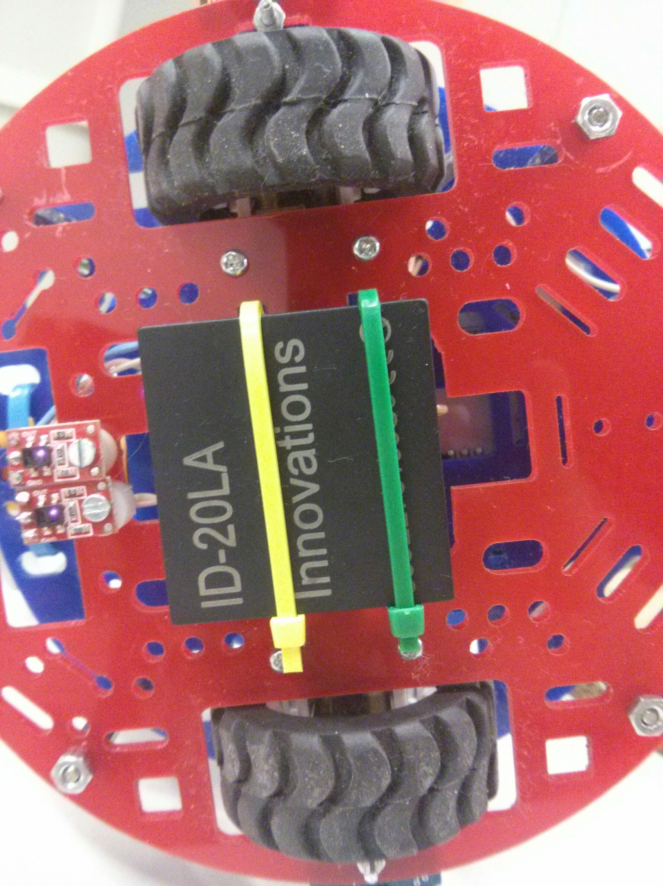
\includegraphics[width=0.3\textheight, angle=-90]{fig/rfid}
	\caption{ID-20LA \acrshort{rfid} reader.}
	\label{fig:rfid}
\end{figure}

On the other hand, there is currently an issue with the availability of the robot. It is powered
with a 2Ah \acrshort{lipo} battery, and is recharged when needed. This has a big issue, since as we
have seen, in high load conditions would not meet the required availability, and furthermore, in
weekends or holidays, there would be no option to change and recharge the battery. Therefore it has
been decided to deploy a cable installation from the ceiling of the laboratory, and the design of
the robot has been adapted so that the cables do not get stuck in the labyrinth.

The rest of the robot will be used as it is, since it provides with the needed capabilities for the
needs of the project: It has a wall sensor capable of avoiding crashes with walls, infrared sensors
to detect the lines in the ground, motors and wheels capable of moving the robot, \acrlong{bt}
connection to communicate with it and an Arduino microcontroller, so that is easy to modify the
current firmware (figure~\ref{fig:bluetooth}).

\begin{figure}[!htbp]
	\centering
	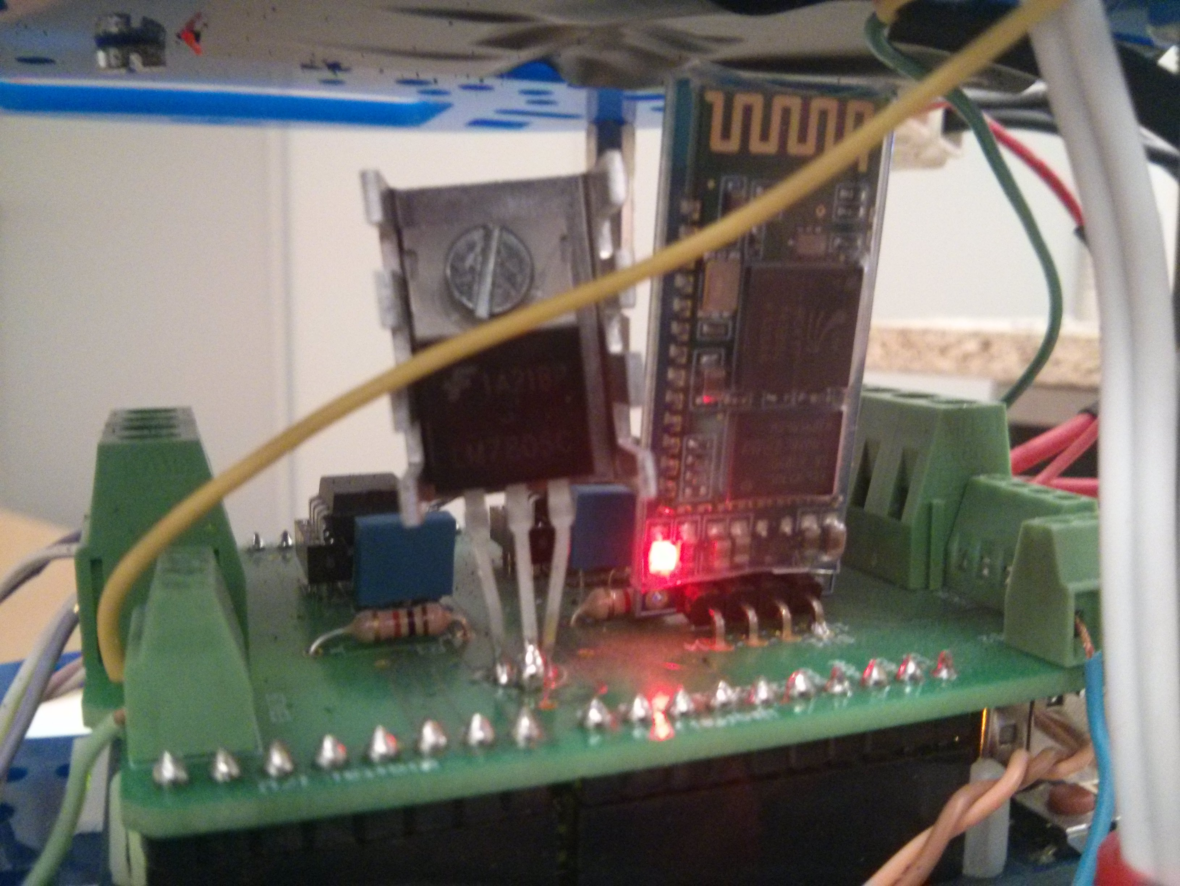
\includegraphics[width=0.65\textwidth]{fig/bluetooth}
	\caption{\acrlong{bt} module on top of the Arduino shield.}
	\label{fig:bluetooth}
\end{figure}

The robot is currently configured with a camera D-link DCS-932L that provides infrared vision if the
light is shut down and normal vision if not, and it can be accessed from Wi-Fi and
Ethernet~\cite{camera}. In this case it will be used via Wi-Fi, since the robot will be moving
around a big space with multiple physical obstacles.

\subsubsection{Software Specification}

The software in for this implementation will be divided modularly, thinking on scalability and
code reuse. The application must be built on top of WebLab-Deusto, so provided \acrshort{api}s will
be used as much as possible. Moreover, and due to deployment needs, the software will be divided
between the robot, an intermediate server and WebLab software. The flow chart for the experiment can
be seen in figure~\ref{fig:exp_flow}. This will be the user's flow in the application. In
figure~\ref{fig:layers} the software layers can be seen, each one with its functions.

\clearpage
\begin{figure}
	\centering
	\includegraphics[width=0.95\textwidth]{fig/experiment-flow}
	\caption{Experiment flow chart.}
	\label{fig:exp_flow}
\end{figure}

\clearpage
\begin{figure}
	\centering
	\includegraphics[width=0.95\textwidth]{fig/layers}
	\caption{Software layers showing each layer's functionality.}
	\label{fig:layers}
\end{figure}
\clearpage

The robot will use a slightly modified version of the current firmware, since it must not get
blocked by any wall in case of crash and a more reliable implementation is needed. That is why it
has been programmed to turn back if a hardware error occurs and collides with a wall. Nevertheless,
the external \acrlong{bt} \acrshort{api} will be the same as the one that was already implemented at
the beginning of the project:

It will provide an ``F'' command to go forward, that will return the \acrshort{rfid} tag if it finds
one, an ``L'' command to turn left, its counterpart ``R'' command to turn right and it will also
provide the command ``S'' that will check if there is a wall in front of the robot. Nevertheless,
and even if the experiment server can check for a wall, the robot itself has been programmed to
return a ``\acrshort{nak}'' response if it is commanded to go forward against a wall.

The robot itself works following the lines in the labyrinth until it finds an intersection. It is
also capable of turning in those intersections: if it is commanded to turn right, it will make a 90
degree right turn and face the path in its right. When the robot stops on top of an \acrshort{rfid}
tag, it will return the tag's label.

The intermediate server will provide a small \acrlong{rest} (\acrshort{rest}) \acrshort{api} in a
small Python server. Its only duty will be to provide a simple interface for the robot using
\acrshort{http} instead of \acrlong{bt}, needed due to deployment constraints. An example of
the \acrshort{api} usage in Python can be seen in algorithm~\ref{alg:romie_rest}.

\begin{center}
\begin{minipage}{.9\textwidth}
\singlespace
\fvset{frame=single}
\begin{pyglist}[language=python, caption={Romie \acrshort{rest} \acrshort{api} example.},
	label={alg:romie_rest}, listingname={Algorithm}, numbers=left]
import urllib2

# Go forward and get RFID tag if exists
tag = urllib2.urlopen('http://192.168.0.190:8000/f',
    timeout = 60).read()

# Left turn
result = urllib2.urlopen('http://192.168.0.190:8000/l',
    timeout = 60).read()

# Right turn
result = urllib2.urlopen('http://192.168.0.190:8000/r',
    timeout = 60).read()

# Check if there is a wall in front of the robot
result = urllib2.urlopen('http://192.168.0.190:8000/s',
    timeout = 60).read()
\end{pyglist}
\fvset{frame=none}
\end{minipage}
\end{center}

This \acrshort{rest} \acrshort{api} is connected to the robot via \acrlong{bt} and sends commands
with the PyBluez \acrlong{bt} wrapper, as it can bee seen in algorithm~\ref{alg:rasp_bluetooth}.
This way, with the software layered, the development is not only faster and easier, but the product
is more scalable and modular.

Then, the experiment server required by the WebLab-Deusto architecture, will provide a WebLab
command \acrshort{api}, that will be callable by the client of the experiment. This server will be
developed in Python because the WebLab Python server libraries are better tested than other language
libraries. The data for the ranking will be stored in a SQLite 3 database. This database provides
all the needed \acrshort{acid} constraints (\acrlong{acid}) with a small \acrshort{sql}
(\acrlong{sql}) \acrlong{rdbms} (\acrshort{rdbms})~\cite{sqlite}.

\begin{center}
\begin{minipage}{.9\textwidth}
\singlespace
\fvset{frame=single}
\begin{pyglist}[language=python, caption={\acrlong{bt} connection example.},
	label={alg:rasp_bluetooth}, listingname={Algorithm}, numbers=left]
try:
    import bluetooth

    BT_address = '00:11:22:33:44:55'
    BT_port = 1

    BT_socket = bluetooth.BluetoothSocket(bluetooth.RFCOMM)
    BT_socket.connect((BT_address, BT_port))

    BT_available = True
except:
    BT_available = False
    print 'No bluetooth device is available'

class RoMIE:
    def _wait_ack(self):
        if not BT_available: return

        # read until ACK or NAK is read
        received = ''
        while 'ACK' not in received and 'NAK' not in received:
            received += BT_socket.recv(1024)
        if 'NAK' in received:
            pass

        return received

    def forward(self):
        if not BT_available: return 'Bluetooth error'

        BT_socket.send('F')
        response = self._wait_ack()
        return response
\end{pyglist}
\fvset{frame=none}
\end{minipage}
\end{center}

The experiment server \acrshort{api} will have all the needed commands to use the experiment. For
the ones that need data being sent to the server, \acrshort{json} has been used (\acrlong{json}). It
is preferred over \acrshort{xml} (\acrlong{xml}) due to the higher compatibility of \acrshort{json}
and the more data-orientation of this \acrlong{rfc} or \acrshort{rfc}. This provides lower
overhead~\cite{xml_vs_json}.

\begin{itemize}
	\item ``\textbf{F}'', ``\textbf{L}'' and ``\textbf{R}'' commands, to move forward and turn left
	and right. The ``S'' command is not provided since the experiment does not require it and the
	robot will not drive towards a wall. The ``\textbf{F}'' will return a random question based on
	the current user's points.

	\item ``\textbf{CHECK\_REGISTER}'' command, to check if the user has been registered in the
	experiment before and decide if the experiment should show the registration form.

	\item ``\textbf{REGISTER}'' command, to send the registration data to the server and insert it
	into the SQLite database.

	\item ``\textbf{ANSWER}'' command, to send the answer given by the user to a question. It will
	return the new date for finishing the experiment and the new points for the user. These will not
	change if the answer was not correct.

	\item ``\textbf{FINISH}'' command, to finish the experiment and receive the final ranking.
\end{itemize}

Finally, the client will be developed using \acrshort{html} 5 (\acrlong{html} version 5),
\acrlong{js} (using JQuery library) and Bootstrap for a rapid development. It will use the WebLab
\acrlong{js} library to communicate with the experiment server. This library is an asynchronous
\acrshort{ajax} (\acrlong{ajax}) library that provides a simple interface to interact with
experiments. An example can be seen in algorithm~\ref{alg:weblab_lib}.

\begin{center}
\begin{minipage}{.9\textwidth}
\singlespace
\fvset{frame=single}
\begin{pyglist}[language=javascript, caption={WebLab \acrlong{js} library example.},
	label={alg:weblab_lib}, listingname={Algorithm}, numbers=left]
// Callback registration that will be
// called after reserving the experiment
Weblab.setOnStartInteractionCallback(start);

// Sending command to the experiment server
Weblab.sendCommand("L", function(response) {
    console.log("Good response: " + response);
}, function(response) {
    console.log("Bad response: " + response);
});
\end{pyglist}
\fvset{frame=none}
\end{minipage}
\end{center}

The game logic is divided between the server and the client. Since the client is manipulable, all
the data is stored in the server and the game cannot be manipulated from client side. This logic
includes the point logic, which has a small bonus depending on when has the last correct answer been
given and the difficulty of the question. An example of this bonus calculation can be seen in the
algorithm~\ref{alg:point_bonus}. As that algorithm shows, the bonus will be a time bonus (the number
of seconds less than 30 since the last correct answer) divided by 5 and multiplied by the difficulty
of the question divided by 10. These bonuses have been adjusted after some trials where they have
been found to enable better gameplay.

\begin{center}
\begin{minipage}{.9\textwidth}
\singlespace
\fvset{frame=single}
\begin{pyglist}[language=python, caption={Point bonus calculation.},
	label={alg:point_bonus}, listingname={Algorithm}, numbers=left]
if correct:
    time_bonus = 30-(time.time()-self.last_correct)
    bonus = (self.q_difficulty/10+1)*
        (time_bonus/5 if time_bonus > 5 else 1)
    self.last_correct = time.time()
    self.points += self.question['points']*bonus
    self.finish_time += self.question['time']*bonus
\end{pyglist}
\fvset{frame=none}
\end{minipage}
\end{center}

After the point calculation, the points in the database get updated. That way, if the user
disconnects from WebLab, or some other issue happens, the points will be saved. Only the best
score is saved. Moreover, and since that database is used for saving the data from the registration
form, which is provided by the user, prepared statements are used in order to avoid \acrshort{sql}
injection attacks.

The game configuration, containing all the questions with their bonuses, the \acrshort{rest}
\acrshort{api} server's \acrshort{ip} and port and all the needed configuration for the display such
as if it is a demonstration environment or needs to show some other client side experiment is stored
in a python file in the experiment server. That way, modifying questions or anything that could be
needed, such as creating debug experiments is managed with that simple configuration script, which
allows for scalability.

Furthermore, since this experiment uses a hardware resource (Romie, the robot), it could happen that
two users try to play with it at the same time. This is solved using the queue management provided
by WebLab. It is as simple as registering the resource's priority queue and WebLab will do all the
needed resource sharing management. Moreover, in the case of having two separate robots of the same
type, it would not be difficult to use the federation model and the user would end up in one of the
two robots transparently.

\subsection{Deployment Considerations}

The deployment must be done in WebLab-Deusto, a remote laboratory environment with three custom
networks and limited physical space. A simplified diagram of the network of WebLab-Deusto can be
seen in figure~\ref{fig:weblab-network}. As that figure shows, Plunder is the core server. It
provides access to WebLab-Deusto web environment and it provides most of the experiment servers. On
the other hand, Blood is the one working as a proxy for all the cameras in WebLab-Deusto, some of
them connected by Wi-Fi and others by Ethernet.

\begin{figure}[!htbp]
	\centering
	\includegraphics[width=0.9\textwidth]{fig/weblab-network}
	\caption{WebLab-Deusto network simplification.}\label{fig:weblab-network}
\end{figure}

In this case, since the use of \acrlong{bt} to connect our experiment server to the robot was a
requirement, and Plunder, Blood and WebLab-test should not receive any new hardware, a Raspberry Pi
Model B computer (figure~\ref{fig:rasp}) will be used, with a \acrshort{usb} (\acrlong{usb})
\acrlong{bt} dongle to connect to the robot and to provide a simple \acrshort{http} server with the
\acrshort{rest} \acrshort{api}. This small computer will be enough for such small web server, since
it provides 512~MB of \acrshort{ram}, a 700~Mhz \acrshort{arm} \acrshort{cpu}, 2 \acrshort{usb}
ports and an Ethernet port. All this in a small form factor, not bigger than a usual credit card,
and consuming only 3.5~W~\cite{rasp_b} of electrical power.

\begin{figure}[!htbp]
	\centering
	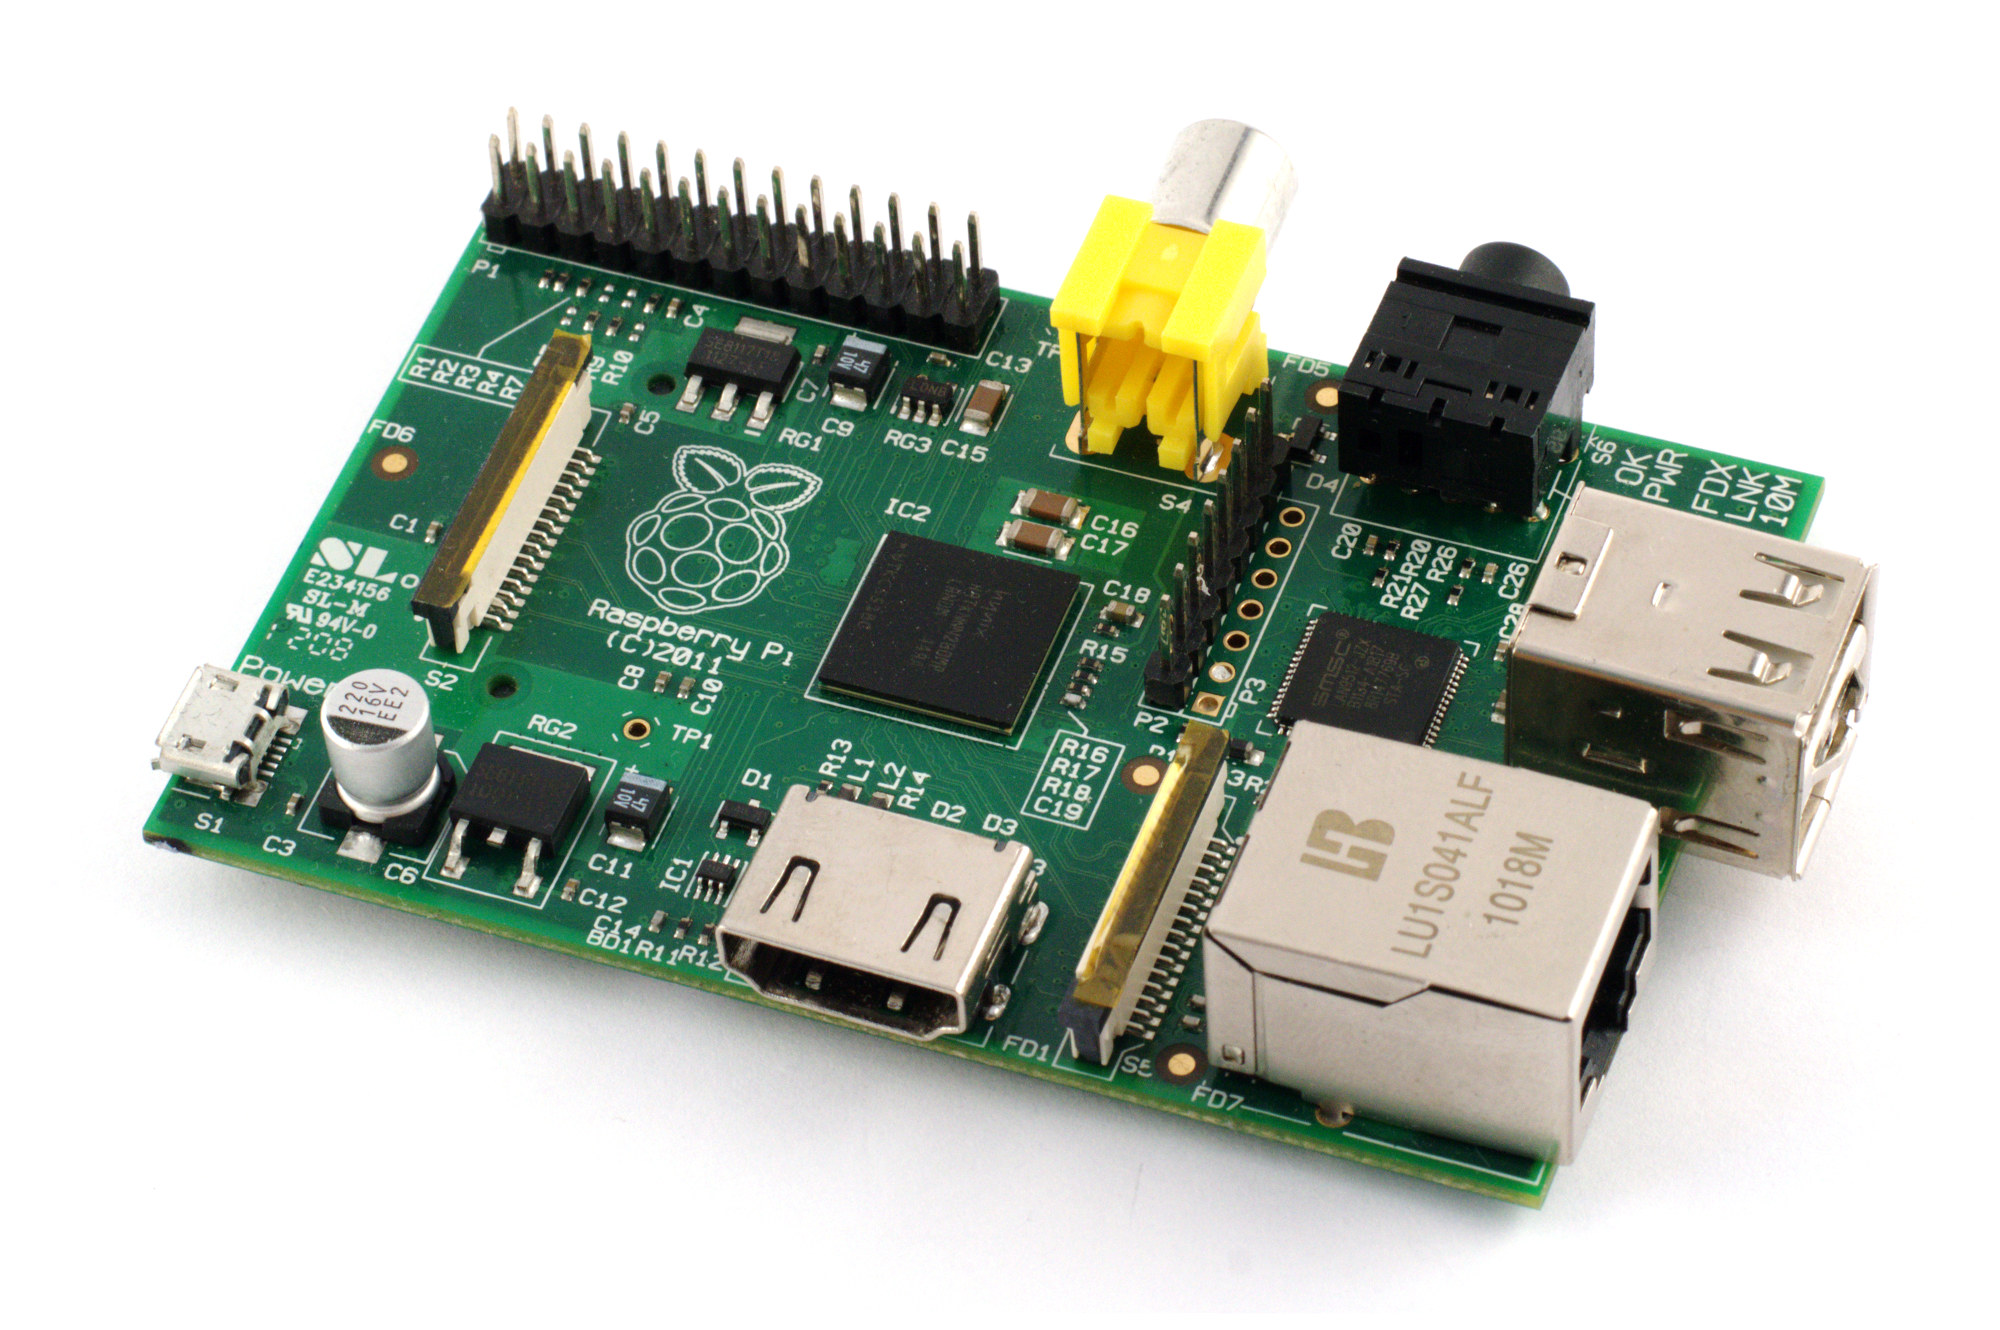
\includegraphics[width=0.7\textwidth]{fig/rasp}
	\caption{Raspberry Pi model B computer.}
	\label{fig:rasp}
\end{figure}

This small computer will be connected via Ethernet to the WebLab network, while two cameras (the top
camera and the on-board camera) will be connected via Wi-Fi to WebLab camera network, using Blood as
the \acrshort{http} proxy server.

Finally, since the server software will change many times during the development, and Plunder must
be restarted for each change if the experiment server is located there, the experiment server for
this experiment will be located in WebLab-test. This way, there will be no need to restart Plunder
each time a new change is made to the experiment, giving higher availability to WebLab-Deusto.

In figure~\ref{fig:labyrinth_diagram} the location of the \acrshort{rfid} tags can be shown in a
scale model of the labyrinth. The labels are these ones, in order:

\begin{itemize}
	\item \textbf{A}: 4F:00:88:AB:CB
	\item \textbf{B}: 4F:00:56:A7:6F
	\item \textbf{C}: 4F:00:56:DA:57
	\item \textbf{D}: 4F:00:56:8F:86
	\item \textbf{E}: 4F:00:56:87:C4
	\item \textbf{F}: 50:00:8F:90:D5
	\item \textbf{G}: 4F:00:56:9F:08
\end{itemize}

\begin{figure}[!htbp]
	\centering
	\includegraphics[width=0.7\textwidth]{fig/labyrinth-diagram}
	\caption{The scale model of the labyrinth used in this project with the \acrshort{rfid} tags.}
	\label{fig:labyrinth_diagram}
\end{figure}

\subsection{Testing Plan}

The testing for this software is divided in 3 main environments. First of all, the usual manual
testing is made by the developers and by the administrators of WebLab-Deusto. This showed many bugs
that they were fixed almost as soon as they appeared, but in any case, this is not enough for a
production environment.

After the manual testing, WebLab-Deusto has a \acrlong{ci} system connected to Travis \acrshort{ci}
in GitHub. It provides many unit tests that provide stability to the code, since the developers
receive emails when a commit does not pass the tests. Nevertheless, for the \acrlong{gui}
(\acrshort{gui}), it is difficult to provide unit tests.

Finally, and also as a demonstration of the potential of the project, the project was tested in an
event at the University of Deusto called ForoTech~\cite{forotech}. In this event the project was
tested in a high load environment, where the robot received hundreds of uses in a short period of
time, demonstrating the reliability and also showing some small issues that were soon fixed.

\subsection{User Manual}

For using Romie, you must have an account in WebLab-Deusto and the appropriate permissions to use
the experiment. Once you fulfill those requirements, go to
\url{https://weblab.deusto.es/weblab/client/}. In that page (figure~\ref{fig:man:weblab}), you will
be able to insert your credentials in the login form and log in.

\begin{figure}[ht]
	\centering
	\includegraphics[width=0.75\textwidth]{fig/manuals/weblab}
	\caption{WebLab Deusto's landing page.}
	\label{fig:man:weblab}
\end{figure}

Once logged in, you will see ``romie'' experiment under the ``Robot experiments'' category
(figure~\ref{fig:man:romie_weblab}). You could see more experiments if you have the permission to
use them. If you cannot find the experiment you should contact with the administrators. Click on
``romie'' or in its image and you will enter the reservation page
(figure~\ref{fig:man:romie_reserve}). There, you can reserve the experiment clicking the ``Reserve''
button.

\begin{figure}[!htbp]
	\centering
	\includegraphics[width=0.85\textwidth]{fig/manuals/trivial/romie-weblab}
	\caption{Romie under ``Robot experiments'' in WebLab Deusto.}
	\label{fig:man:romie_weblab}
\end{figure}

\begin{figure}[!htbp]
	\centering
	\includegraphics[width=0.5\textwidth]{fig/manuals/trivial/romie-reserve}
	\caption{Romie reservation screen.}
	\label{fig:man:romie_reserve}
\end{figure}

Once reserved, on the first use, you will see the registration form
(figure~\ref{fig:man:romie_register}). You will have to fill it in order to play the game. There is
also a version without the registration screen if you only want to test the robot, ask the
administrators for permission to use it. After filling the registration form  with your own data,
you can click the register button. \emph{Note: the experiment is prepared to work with students of
less than 18 years old, so any age above that or below 5 years old is considered an input error,
that will be notified in the \acrlong{ui}}.

\begin{figure}[!htbp]
	\centering
	\includegraphics[width=0.85\textwidth]{fig/manuals/trivial/romie-register}
	\caption{Romie's registration form.}
	\label{fig:man:romie_register}
\end{figure}

After the registration, you will be able to play with Romie. The game is pretty easy to use: you
will have three arrows in the left control pad (figure~\ref{fig:man:romie_start}), where you will be
able to click and command the robot to move forward or to turn left or right. Moreover, you will
have the on-board camera to see what the robot does. If you press forward against a wall do not
worry, the robot will not collide.

\begin{figure}[!htbp]
	\centering
	\includegraphics[width=0.85\textwidth]{fig/manuals/trivial/romie-start}
	\caption{Playing with Romie.}
	\label{fig:man:romie_start}
\end{figure}

If you fall in top of a card, you will be asked a question (figure~\ref{fig:man:romie_question}). If
you answer correctly, you will be given points and more time to continue playing. Furthermore, you
will have the opportunity to manually activate the ceiling camera to see all the labyrinth and
decide where to go (figure~\ref{fig:man:romie_ceiling}).

\begin{figure}[!htbp]
	\centering
	\includegraphics[width=0.85\textwidth]{fig/manuals/trivial/romie-question}
	\caption{Romie asks you questions when you drive onto a card.}
	\label{fig:man:romie_question}
\end{figure}

\begin{figure}[!htbp]
	\centering
	\includegraphics[width=0.85\textwidth]{fig/manuals/trivial/romie-ceiling}
	\caption{You can activate the ceiling camera when you answer a question correctly.}
	\label{fig:man:romie_ceiling}
\end{figure}

Finally, when the time finishes, you will see a ranking with the 10 best scores of the game (less if
there has not been enough users) with your user selected in green if you are in the top ten, as you
can see in figure~\ref{fig:man:romie_ranking}.

\begin{figure}[!htbp]
	\centering
	\includegraphics[width=0.85\textwidth]{fig/manuals/trivial/romie-ranking}
	\caption{The final ranking where you can see the best scores.}
	\label{fig:man:romie_ranking}
\end{figure}

\subsection{Issue Management}

During the development some issues have been faced, which had to be solved. One of the first issues
that appeared was that the robot was not reading the lines properly, mainly the ones in the
intersections. That was caused because the contrast between the line and the background was
insufficient. It was solved by painting all the labyrinth in white and painting the black lines.
That way there was no need for using tape and the robot started to work properly.

Other issue that came across was that the robot did not read the \acrshort{rfid} tags every time it
went on top of them. The problem was that the \acrshort{rfid} reader the robot had, the ID-12 seemed
to have some defect, since the reader was located about 10-15~mm from the floor and its range was of
120~mm~\cite{rfid}. It was decided to change it by a ID-20 reader, that has a 180~mm
range~\cite{rfid} and worked perfectly.

\begin{figure}[!htbp]
	\centering
	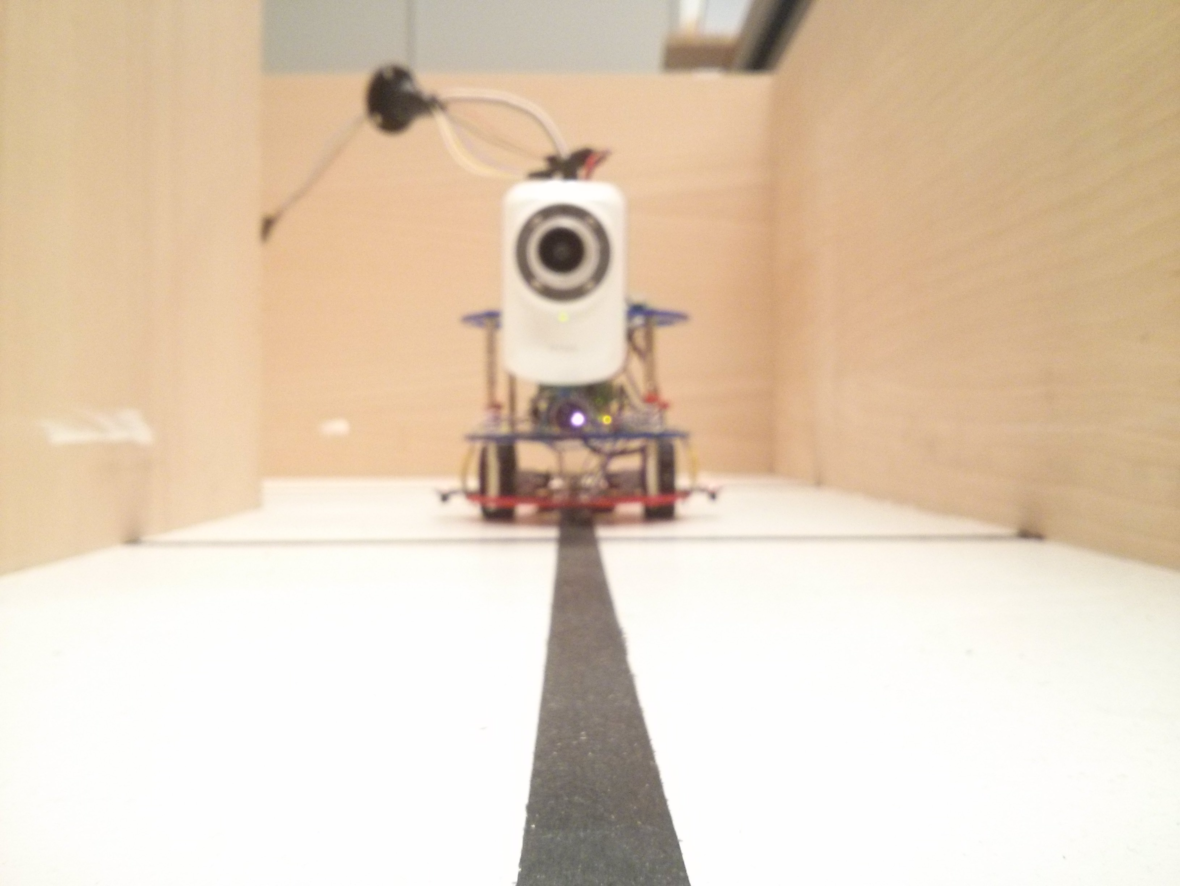
\includegraphics[height=0.35\textheight]{fig/lines}
	\caption{Romie must not get entangled with the walls.}
	\label{fig:lines}
\end{figure}

Furthermore, the electricity was another problem: the robot was using batteries, and as it can be
seen above, it had to be changed to cables. The main issue was that the cables could get entangled
with the walls. It was solved by extending a flexible artifact in top of the robot
(figure~\ref{fig:lines}).

\begin{center}
\begin{minipage}{.9\textwidth}
\singlespace
\fvset{frame=single}
\begin{pyglist}[language=c, caption={Arduino code for returning if wall was hit.},
	label={alg:romie_wall}, listingname={Algorithm}, numbers=left]
if (millis()-lastTimeFollow >= 8000) {
    while(digitalRead(FLIline) == HIGH) Motors.turnRight(100);
    while(digitalRead(FRIline) == LOW) Motors.turnRight(100);
    FollowLine();
    lastTimeFollow=millis();
}
\end{pyglist}
\fvset{frame=none}
\end{minipage}
\end{center}

Finally, there was a problem with the wall sensor, since it would disconnect sometimes. This was a
hardware issue that could not be solved easily, since the sensor would arrive at least 1 month after
being requested. Taking that into account it was decided to implement a software solution directly
in the robot so that it would go back automatically if something went wrong, as it can be seen in
algorithm~\ref{alg:romie_wall}.

\subsection{Labpsico Experiment Integration}

When the trivial type game was almost finished, there was an opportunity to work with Deusto's
psychology laboratory, Labpsico. They proposed to integrate an experiment they had with this game,
so that users could perform their activity before playing.

This experiment had been developed by Helena Matute's team, recently prized by the Jot Down
magazine~\cite{jotdown_helena} by one of her works. The experiment consists on clicking in 40 cards
and looking on the other side of them. Randomly, a mark can appear in one or both sides of the card
(figure~\ref{subfig:labpsico_card_mark}) and users should be able to determine if there is
correlation between the two marks.

\begin{figure}[!htbp]
	\centering
	\begin{subfigure}{0.4\textwidth}
		\centering
		\includegraphics[height=0.3\textheight]{fig/manuals/trivial/labpsico/card1}
		\caption{Labpsico card without a mark}\label{subfig:labpsico_card}
	\end{subfigure}\quad
	\begin{subfigure}{0.4\textwidth}
		\centering
		\includegraphics[height=0.3\textheight]{fig/manuals/trivial/labpsico/card2}
		\caption{Labpsico card with a mark.}\label{subfig:labpsico_card_mark}
	\end{subfigure}\quad
	\caption{Some of the cards used in Labpsico's experiment.}
\end{figure}

After that, the users will be divided into two groups: test users and control users. This way, using
the blind experiment technique, they will show some random information to the control group and
information about medicine effectiveness to the test group. Then they will repeat the experiment
using some other cards but with the same randomness.

Comparing both experiments Labpsico will get the real knowledge of how did the experience change
their minds about not proven science or \emph{pseudoscience}. After that, a score will be given to
the user that will be added to the game (figure~\ref{fig:labpsico_romie}).

\begin{figure}[ht]
	\centering
	\includegraphics[height=0.35\textheight]{fig/manuals/trivial/labpsico/labpsico-romie}
	\caption{Romie game with the Labpsico experiment.}
	\label{fig:labpsico_romie}
\end{figure}

For the integration of this experiment, and since it has been developed using Bootstrap, there is no
need on changing its style. Moreover, there were tight style requirements from the Labpsico team, so
this could not be changed easily. That is why only some of the libraries have been modified to take
benefit from the ones already used in WebLab and to lower the number of downloads per request.
Finally, a simple \emph{iframe} \acrshort{html} element has been used to show the experiment inside
the Bootstrap's \emph{modal} element. The data is sent to Labpsico directly using the web interface,
using an on-line database in FireBase~\cite{firebase}. This experiment will only appear once per
each user.

\FloatBarrier
\clearpage
\section{Visual Programming}

The second part of this project is to develop a visual programming interface to program the robot
and test the programming skills of the users. Since the hardware platform for this section has been
the same as for the trivial type game, hardware requirements are not included in this section.
Furthermore, since the same software design is followed for the communication with the robot, there
is no need on adding it to this section.

We will therefore explain the software requirements for the visual programming client, the design
specification of the software that has been used for this section and the user manual for this
application, along with the issue management of this section, that will be mainly focused on the
software issues.

There is no need of explaining the testing plan, since it has been the same as the one used in the
trivial game, except from the real user testing, that we have not been able to do.

\subsection{Software Requirements}

The software requirements of this application will be based on usability, minimal WebLab resource
usage and effectiveness of the programming. Those requirements are listed below:

\begin{itemize}

	\item The user interface must allow the user to understand how to program the robot.
	\item The user interface must show the robot doing what had been programmed to do.
	\item The robot must follow the code developed in the interface.
	\item The programming must not block the interface of the user.
	\item The program development must not use the resource until the test is reserved.
	\item The user must be able to edit the program after testing it.
	\item The server and the client must be loosely coupled.

\end{itemize}

Taking into account those requirements, it has been decided to develop a new experiment server and
to add some more \acrshort{api}s to WebLab client. Moreover, Google's Blockly~\cite{blockly} is
going to be used for the development, since it is the most known platform to create visual editors
in a web platform and contains code generators for \acrlong{js}, Dart~\cite{dart}, Python and
\acrshort{php}.

\subsection{Design Specification}

The software itself will follow the same design specification as in the trivial game. Nevertheless,
it has been decided that the code generation is going to be done in the client side, since it
supposes less security concern by using the \acrshort{api} provided by the experiment server and not
programming the experiment server itself (or even the robot). Therefore, \acrlong{js} generator will
be used.

Moreover, since one of the requirements is that the software must not use the resource (the robot
Romie) while the user is creating the program, and can only be reserved once the user tries to test
it, a new \acrshort{api} call is needed in the WebLab \acrshort{api}. We can see an example of this
\acrshort{api} calls in the algorithm~\ref{alg:new_api}.

\begin{center}
\begin{minipage}{.9\textwidth}
\singlespace
\fvset{frame=single}
\begin{pyglist}[language=javascript, caption={New WebLab \acrshort{api} functions.},
	label={alg:new_api}, listingname={Algorithm}, numbers=left]
// We set a callback for being called when reserving the experiment.
//
// This way, the server will be able to know the program and
// return it to the client once the experiment is reserved.
Weblab.setOnGetInitialDataCallback(function() {
    return {"blocks": Blockly.Xml.domToText(
        Blockly.Xml.workspaceToDom(workspace)
    )};
});

// We set a callback for finishing the experiment.
//
// This way, we can save the data into web storage
// and enable the user to edit the code and reserve
// again.
Weblab.setOnFinishedCallback(function(data) {
    console.log("Experiment finished with: ");
    console.log(data);
});
\end{pyglist}
\fvset{frame=none}
\end{minipage}
\end{center}

Moreover, since all commands in WebLab are sent asynchronously, we need to wait for the movement to
finish before attempting the next movement. The problem is that if we do a \emph{while} loop, the
interface will be broken in an infinite loop. In this case, we have taken advantages of the scopes
introduced by the \acrshort{js}-interpreter and we have created some wrapper functions to move the
robot. We can see the real function example in algorithm~\ref{alg:move_func}, the wrapper function
example in algorythm~\ref{alg:wrapper} and the generated code in algorithm~\ref{alg:generated}.

As we can see, we first define the move functions in a similar way to what we did for the trivial
type game. Then, we create some wrappers for the functions and add them to the context of the code
execution. That way, in out block code we can call those functions and not block the execution, so
that we can do a \emph{while} loop until the server responds.

\begin{center}
\begin{minipage}{.9\textwidth}
\singlespace
\fvset{frame=single}
\begin{pyglist}[language=javascript, caption={Robot movement function.},
	label={alg:move_func}, listingname={Algorithm}, numbers=left]
Romie = function() {
    this.moving = false;
}

Romie.prototype.forward = function() {
    this.moving = true;
    Weblab.sendCommand('{"command":"F"}', function(response) {
        this.moving = false;
    }.bind(this));
}

var romie = new Romie();
\end{pyglist}
\fvset{frame=none}
\end{minipage}
\end{center}

\begin{center}
\begin{minipage}{.9\textwidth}
\singlespace
\fvset{frame=single}
\begin{pyglist}[language=javascript, caption={Function wrapper.},
	label={alg:wrapper}, listingname={Algorithm}, numbers=left]
function initApi(interpreter, scope) {
	// Add Romie movement checker to the context
	var wrapper = function() {
		return interpreter.createPrimitive(romie.isMoving());
	};
	this.setProperty(scope, 'isMoving',
		this.createNativeFunction(wrapper));

	// Add an API function for the forward() block.
	wrapper = function() {
		romie.forward();
	};
	interpreter.setProperty(scope, 'forward',
		interpreter.createNativeFunction(wrapper));
}
var myInterpreter = new Interpreter(
	Blockly.JavaScript.workspaceToCode(workspace),
	initApi);
\end{pyglist}
\fvset{frame=none}
\end{minipage}
\end{center}

\begin{center}
\begin{minipage}{.9\textwidth}
\singlespace
\fvset{frame=single}
\begin{pyglist}[language=javascript, caption={Generated code.},
	label={alg:generated}, listingname={Algorithm}, numbers=left]
// Block code
Blockly.JavaScript['romie_move_forward'] = function(block) {
    code = 'forward();\n'+
            'while(isMoving());\n';
    return code;
};

// Which generates
forward();
while(isMoving());
\end{pyglist}
\fvset{frame=none}
\end{minipage}
\end{center}

Since one of the requirements is for the user to always know what is happening, we will use the
block highlighting provided by blockly. This way, when the code is executed, the code being executed
is highlighted, and the user can debug the code.

Furthermore, the user interface displays the two cameras of the robot once it starts testing the
code. This way, the user can see what is happening with the robot and actually test how the robot
moves.

TODO: experiment flow

\subsection{User Manual}

TODO: user manual

\subsection{Issue Management}

TODO: issue management

\FloatBarrier
\section{Technology}

In this section we will analyze the technology and tools used for this project. The technology has
been divided between hardware and software, since in this project, both aspects have had big impact.

\subsection{Hardware}

In this case, the hardware has been divided in mainly two parts. First of all, the hardware used by
the robot itself, has been the Arduino Uno microcontroller (figure~\ref{fig:arduino_board}. This
microcontroller provides the ATmega328 microcontroller with 14 digital input/output pins, 6 analog
inputs and a \acrshort{usb} connector~\cite{arduino_datasheet}.

\begin{figure}[!htbp]
	\centering
	\includegraphics[height=0.3\textheight]{fig/arduino-board}
	\caption{Arduino Uno microcontroler.}
	\label{fig:arduino_board}
\end{figure}

The hardware attached to the Arduino Uno is mainly the same it had when the project started. A
\emph{E18-D80NK} infrared adjustable sensor for wall sensing, \emph{MSE-S110.2} sensors for
following the line, a \emph{Grove Line Finder} for detecting intersections, a
\emph{BT Board v1.02} Bluetooth adapter for Bluetooth communication~\cite{fdp_itu}. The
\acrshort{rfid} reader, on the other hand, and as we have seen before, has been changed by an
ID-20~\cite{rfid} sensor, since the ID-12 we had was not working properly.

For the \acrshort{http} server, a Raspberry Pi model B has been used. The reason for not using the
model B+ or the Raspberry Pi 2 model B has been that we already had an unused Raspberry Pi model B
in WebLab-Deusto. and this hardware was enough to provide the services needed by this project. This
computer has been used as a client connected via Bluetooth to the robot and as a server connected
via Ethernet to the WebLab-Deusto network. Raspberry Pi foundation (figure~\ref{fig:rasp_logo})
develops these tiny computers to teach kids about computers and programming in a very affordable
way.

\begin{figure}[!htbp]
	\centering
	\includegraphics[width=0.2\textwidth]{fig/rasp-logo}
	\caption{Raspberry Pi logo.}
	\label{fig:rasp_logo}
\end{figure}

\subsection{Software}

In this project, since we have integrated many hardware and software technologies, we have used many
software platform and languages. Some of them were new, while others were known. The core
functionality of the project has been developed in JavaScript for the client side and Python for the
server side.

TODO: Python, HTML 5, JavaScript, WebLab, JSON, HTTP, REST, Bluetooth,

\section{Tools}

\subsection{Code editor}

For developing this project, some tools have been used. We will analyze them here and see why they
have been used.

The first tool used has been the code editor. The editor used has been Sublime
Text~\cite{sublime_web}. We were using version 2 until March 2015, where development in version 3
gave life signs and we decided to upgrade the version. There are multiple \acrshort{ide}s such as
PyCharm~\cite{pycharm_web}, Eclipse~\cite{eclipse_web} or other editors such as
Atom~\cite{atom_web}, Lime Text~\cite{lime_web} or Microsoft Visual Studio Code~\cite{ms_code_web}.
There are also other console tools like Vim~\cite{vim_web}, Nano~\cite{nano_web} or
Emacs~\cite{emacs_web}.

Nevertheless, even if I would have preferred to work with an open source editor, the truth is that
currently, the closed sourced ones offer better performance. For instance, Atom tries to be the
open source alternative to Sublime Text, but it starts really slowly and the plug-ins for Sublime
Text can be found for almost every situation. Lime Text might outperform Sublime Text in the future
but currently it is still in an unstable release. Microsoft Visual Studio Code was released later
this year and it did not have any benefit with respect to Sublime Text, so it was worthless changing
the editor at this point.

\begin{figure}[!htbp]
	\centering
	\begin{subfigure}{0.35\textwidth}
		\centering
		\includegraphics[width=0.6\textwidth]{fig/sublime}
		\caption{Sublime Text logo.}\label{subfig:sublime}
	\end{subfigure}\quad
	\begin{subfigure}{0.55\textwidth}
		\centering
		\includegraphics[width=0.7\textwidth]{fig/arduino-community}
		\caption{Arduino Community logo. \emph{Source: Arduino}}\label{subfig:arduino_community}
	\end{subfigure}\quad
	\caption{Code editors used.}
\end{figure}

On the other hand, \acrshort{ide}s are big softwares that from my point of view interfere in the
programming process. In the end, this is about feeling comfortable with the tool, and the velocity
and simplicity offered by editors outperform \acrshort{ide}s greatly. That is why the tool used for
all the programming (except the Arduino script) has been Sublime Text 3
(figure~\ref{subfig:sublime}).

Nevertheless, since the robot's microcontroller is an Arduino, the Arduino
\acrshort{ide}~\cite{arduino_ide} (figure~\ref{subfig:arduino_community}) has been used to program
the robot itself, since it is simple and easy to use for this simple task. For some specific
situations such as small testing changes made in the project's Raspberry Pi or testing server
configuration Nano has been used since it provides a simple console interface easy to use when
connecting via \acrshort{ssh} (\acrlong{ssh}).

\subsection{User interface testing}

Since one of the key points of the project has been the user interface and in overall the web client
of the system, this needed to be tested. For this task, two main web browsers have been used:
Mozilla Firefox~\cite{firefox_web} (figure~\ref{subfig:firefox}) and Google Chrome~\cite{chrome_web}
(figure~\ref{subfig:chrome}). Here, it has been found that Google Chrome's developer tools have
helped the development more, thanks to their features and ease of use. We can see a screenshot of
Google Chrome's developer tools in figure~\ref{fig:chrome_dev}.

\begin{figure}[!htbp]
	\centering
	\begin{subfigure}{0.45\textwidth}
		\centering
		\includegraphics[width=0.5\textwidth]{fig/firefox}
		\caption{Mozilla Firefox logo.}\label{subfig:firefox}
	\end{subfigure}\quad
	\begin{subfigure}{0.45\textwidth}
		\centering
		\includegraphics[width=0.5\textwidth]{fig/chrome}
		\caption{Google Chrome's logo.}\label{subfig:chrome}
	\end{subfigure}\quad
	\caption{Web browsers used for testing.}
\end{figure}

\begin{figure}[!htbp]
	\centering
	\includegraphics[width=0.95\textwidth]{fig/chrome-dev}
	\caption{Google Chrome's developer tools.}
	\label{fig:chrome_dev}
\end{figure}

\subsection{Operating system and tools}

For the development, the \acrlong{os} used has been Ubuntu \acrshort{gnome}~\cite{ubuntu_gnome_web}
(figure~\ref{subfig:ubuntu_gnome}). This distribution gives all the needed productivity and user
friendliness. The user interface used has been \acrshort{gnome} Shell, and as far as possible, it
has been tried to use only \acrshort{floss} software (\acrlong{floss}).

Moreover, for the server environments two main operating systems have been used: Ubuntu
Server~\cite{ubuntu_web} (figure~\ref{subfig:ubuntu}) and Raspbian~\cite{raspbian_web}, the
Raspberry Pi \acrshort{arm} compatible Debian~\cite{debian_web} distribution
(figure~\ref{subfig:debian}). The first of the two has been used for main WebLab-Deusto servers. It
is used due to its user friendliness, even if being a \acrshort{cli} interface (\acrlong{cli}). The
second one has been used due to its compatibility with the hardware being used for the project, the
Raspberry Pi computer.

\begin{figure}[!htbp]
	\centering
	\begin{subfigure}{0.3\textwidth}
		\centering
		
\includegraphics[width=0.6\textwidth]{fig/ubuntu-gnome}
		\caption{Ubuntu \acrshort{gnome} logo.}\label{subfig:ubuntu_gnome}
	\end{subfigure}\quad
	\begin{subfigure}{0.3\textwidth}
		\centering
		\includegraphics[width=0.6\textwidth]{fig/ubuntu}
		\caption{Ubuntu logo.}\label{subfig:ubuntu}
	\end{subfigure}\quad
	\begin{subfigure}{0.3\textwidth}
		\centering
		\includegraphics[width=0.5\textwidth]{fig/debian}
		\caption{Debian logo.}\label{subfig:debian}
	\end{subfigure}\quad
	\caption{Operating systems used in this project.}
\end{figure}

In all cases, the communication between the various servers has been done via \acrshort{ssh}, since
it provides an easy interface with the consoles of the servers.

\subsection{Version control}

For the version control of the project, Git~\cite{git_web} has been used (figure~\ref{subfig:git}).
Git is a distributed \acrlong{vcs} or \acrshort{vcs} created by Linus Torvalds to improve the Linux
kernel development. It allows having repositories distributed without a need of a central
repository. Nevertheless, we have used GitHub~\cite{github_web} for the Git hosting as well as for
issue tracking since GitHub provides with a simple issue management interface, with integrated pull
requests, simple and effective.

\begin{figure}[!htbp]
	\centering
	\begin{subfigure}{0.6\textwidth}
		\centering
		\includegraphics[width=0.6\textwidth]{fig/git.eps}
		\caption{Git logo.}\label{subfig:git}
	\end{subfigure}\quad
	\begin{subfigure}{0.3\textwidth}
		\centering
		\includegraphics[width=0.55\textwidth]{fig/github}
		\caption{GitHub's octocat logo.}\label{subfig:github}
	\end{subfigure}\quad
	\caption{Tools and services used for version control.}
\end{figure}


\chapter{Conclusions and Future Work}

\section{Conclusions}

TODO: Conclusions

\section{Future Work}

TODO: Future Work


\printbibliography[heading=bibintoc]
\printglossary[type=\acronymtype]

\appendix

\chapter*{Acknowledgements}
\addcontentsline{toc}{chapter}{Acknowledgements}

I would like to thank the following people for their help, since without them this project would not
have been possible. Thanks to them I was able to life this amazing experience.

\begin{itemize}
	\item \textbf{My mum, Arantza}, for dedicating her last days of her life to support me when I
	was starting my first months of my degree, and for being the best mother any kid could dream of.

	\item \textbf{My dad, Manu}, for being patient with me all these years and giving me the
	opportunity to continue my studies by giving me moral and financial support.

	\item \textbf{Javier García Zubía}, for being the tutor of this project and for giving me the
	opportunity to learn while working in WebLab-Deusto for the last two years.

	\item \textbf{Helena Matute}, for giving me the opportunity to work in collaboration with the
	Labpsico team and create an awesome experience.

	\item \textbf{Tomás de la Vega}, for being so receptive with my inquiries when integrating the
	Labpsico experiment.

	\item \textbf{Pablo Garaizar \emph{``Txipi''}}, for recommending me to Javier García Zubía as a
	potential candidate to work in WebLab-Deusto.

	\item \textbf{Pablo Orduña}, for letting me understand \emph{his} WebLab-Deusto and helping me
	each time I had issues in my development.

	\item \textbf{Luis Rodríguez}, for being incredibly patient with all my questions, that were not
	few.

	\item \textbf{Gabriel Martinez}, for having him in WebLab-Deusto and for being a good co-worker.
	His contributions to the \acrshort{ai} of the robot were priceless.

	\item \textbf{Ignacio Angulo}, for helping me with the electronics of the robot. I was able to
	learn a lot with him.
\end{itemize}

\chapter*{Agradecimientos}
\addcontentsline{toc}{chapter}{Agradecimientos}

Me gustaría agradecer a las siguientes personas por su ayuda, ya que sin ellas este proyecto no
habría sido posible. Gracias a ellos pude vivir esta asombrosa experiencia.

\begin{itemize}
	\item \textbf{Mi madre, Arantza}, por dedicar sus últimos días de su vida a apoyarme cuando
	comenzaba mis primeros meses de carrera, y por ser la mejor madre que ningún niño podría soñar.

	\item \textbf{Mi padre, Manu}, por ser paciente conmigo todos estos años y haberme dado la
	oportunidad de continuar mis estudios dándome a su apoyo moral y financiero.

	\item \textbf{Javier García Zubía}, por ser el tutor de este proyecto y por darme la oportunidad
	de aprender mientras trabajaba en WebLab-Deusto los últimos dos años.

	\item \textbf{Helena Matute}, por darme la oportunidad de trabajar en colaboración con el equipo
	de Labpsico y crear una experiencia sorprendente.

	\item \textbf{Tomás de la Vega}, por ser tan receptivo con mis consultas al integrar el
	experimento de Labpsico.

	\item \textbf{Pablo Garaizar \emph{``Txipi''}}, por recomendarme a Javier García Zubía como un
	candidato potencial para trabajar en WebLab-Deusto.

	\item \textbf{Pablo Orduña}, por permitirme entender \emph{su} WebLab-Deusto y ayudarme cada
	vez que tenía problemas con el desarrollo.

	\item \textbf{Luis Rodríguez}, por ser increíblemente paciente con todas mis preguntas, que no
	fueron pocas.

	\item \textbf{Gabriel Martinez}, por tenerlo en WebLab-Deusto y ser un buen compañero de
	trabajo. Sus contribuciones a la \acrshort{ia} del robot fueron impagables.

	\item \textbf{Ignacio Angulo}, por ayudarme con la electrónica del robot. Con el pude aprender
	mucho.
\end{itemize}


\backmatter

\end{document}
